\documentclass[bsc, frontabs, twoside, singlespacing, parskip]{infthesis}

\usepackage{amsmath}
\usepackage{graphicx}
\usepackage{url}
%\usepackage[font=small,format=plain,labelfont=bf,up,textfont=it,up]{caption}
%\usepackage{fullpage}
%\usepackage{parskip}
\usepackage{listings}
\usepackage{color}
\usepackage{subcaption}
\usepackage{acronym}
\usepackage{todonotes}

\let\oldtodo\todo
\newcommand{\tdi}[1]{\oldtodo[inline]{#1}}
\renewcommand\todo[1]{\oldtodo[size=\tiny]{#1}}
\newcommand{\tdic}[2][]{
    \oldtodo[inline, caption={#1}]{
        \begin{minipage}{
            \textwidth-4pt
        }
        #2
        \end{minipage}
    }
}
\setlength{\marginparwidth}{2cm}

\definecolor{mygreen}{rgb}{0,0.6,0}
\definecolor{mygray}{rgb}{0.5,0.5,0.5}
\definecolor{mymauve}{rgb}{0.58,0,0.82}

\lstset{ %
  backgroundcolor=\color{white},   % choose the background color; you must add \usepackage{color} or \usepackage{xcolor}
  basicstyle=\footnotesize,        % the size of the fonts that are used for the code
  breakatwhitespace=false,         % sets if automatic breaks should only happen at whitespace
  breaklines=true,                 % sets automatic line breaking
  captionpos=b,                    % sets the caption-position to bottom
  commentstyle=\color{mygreen},    % comment style
  deletekeywords={...},            % if you want to delete keywords from the given language
  escapeinside={\%*}{*)},          % if you want to add LaTeX within your code
  extendedchars=true,              % lets you use non-ASCII characters; for 8-bits encodings only, does not work with UTF-8
  keywordstyle=\color{blue},       % keyword style
  language=Python,                 % the language of the code
  morekeywords={*,...},            % if you want to add more keywords to the set
  numbers=left,                    % where to put the line-numbers; possible values are (none, left, right)
  numbersep=5pt,                   % how far the line-numbers are from the code
  numberstyle=\tiny\color{mygray}, % the style that is used for the line-numbers
  rulecolor=\color{black},         % if not set, the frame-color may be changed on line-breaks within not-black text (e.g. comments (green here))
  showspaces=false,                % show spaces everywhere adding particular underscores; it overrides 'showstringspaces'
  showstringspaces=false,          % underline spaces within strings only
  showtabs=false,                  % show tabs within strings adding particular underscores
  stepnumber=1,                    % the step between two line-numbers. If it's 1, each line will be numbered
  stringstyle=\color{mymauve},     % string literal style
  tabsize=2,                       % sets default tabsize to 2 spaces
}

\acrodef{UI}{User Interface}
\acrodef{UX}{User Experience}
\acrodef{tf.idf}{term frequency-inverse document frequency}
\acrodef{GUI}{Graphical User Interface}
\acrodef{API}{Application Programming Interface}

\begin{document}

\title{A Tool for Visualising Cell Model Results \\
       MInf Project Phase 2}
\author{James Hulme}
\course{Master of Informatics}
\project{MInf Project (Part 2) Report}
\abstract{This will be the abstract}

\maketitle

\section*{Acknowledgements}
Acknowledgements go here.

\thispagestyle{empty}

\newpage

%\begin{abstract}
%This is where the abstract will go
%\end{abstract}

\thispagestyle{empty}

\newpage

\tableofcontents
\thispagestyle{empty}

\clearpage
\setcounter{page}{1}

\section{Introduction}

Biologists often use computer models to help guide their research as modelling is much cheaper than experimentation.  There are a number of tools available for biological modelling.  These tools typically require a certain level of numerical confidence to create and interpret.  Not all biologists have this numerical confidence.  Some researchers find writing and interpreting models a challenge, this can make them less effective in their research.  It is therefore necessary for the tools they use to help them relate the data to their field by incorporating domain knowledge.

One such tool that can be used for modelling is Bio-PEPA, an extension of the PEPA process algebra.  Bio-PEPA is currently implemented as a plugin for the Eclipse IDE.  Bio-PEPA visualises the model results as time-series graphs.  There is one team, of Src researchers, in particular who use Bio-PEPA and do not have the numerical confidence, as described above, to be comfortable using Bio-PEPA.  This team is the focus for this project.  The purpose of this project was to extend Bio-PEPA's visualisation capabilities to allow the previously mentioned team, and other similar users of Bio-PEPA to more effectively analyse their results.

A significant problem with Bio-PEPA's visualisation capability is that it is difficult to represent spatial change on a time-series graph (as can be seen in Figure~\ref{fig:asrc_intro}).  In Bio-PEPA you can have a species at different locations in the cell, for example, next to the nucleus, next to the cell membrane and throughout the cytoplasm.  The movement of this species through the cell can by modelled by seeing the population of it in each location over time.  This is difficult to visualise on a time series plot as three lines is too abstract.  It requires the use of biological metaphor to be easily interpreted.  In this case using visualisation based on a cell can more intuitively show how the species moves through the cell.  It is this sort of inference that the Src researches find challenging to do with Bio-PEPA currently.

\begin{figure}[h!]
    \centering
    \begin{subfigure}[b]{0.4\textwidth}
        \centering
        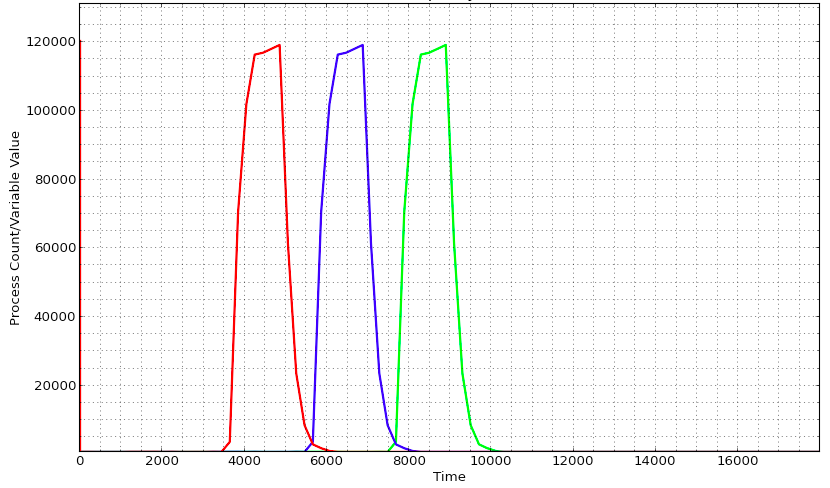
\includegraphics[width=0.8\textwidth]{images/asrc_graph_intro.png}
        \caption{Time Series Representation}
        \label{fig:asrc_graph_intro}
    \end{subfigure}
    \begin{subfigure}[b]{0.4\textwidth}
        \centering
        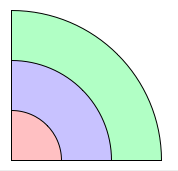
\includegraphics[width=0.5\textwidth]{images/asrc_cell_intro.png}
        \caption{Spatial Representation}
        \label{fig:asrc_cell_intro}
    \end{subfigure}
    \caption{One species at three locations in the cell represented traditionally on a time series graph and also spatially in a cell}
    \label{fig:asrc_intro}
\end{figure}


Over the course of the project the scope has been expanded.  The original objective was to assess which forms of visual representation are most helpful and informative to laboratory science.  At the end of the first project phase the object changed (to reflect that the project was about delivering a finished program the results of many experiments) to be to develop a tool to visualise the results of dynamic, time-series models of intra-cellular behaviour based on biochemical reactions.  This objective was focused on visualisation to aid those researchers who are not numerically confident.  The second phase of the project has added to this objective to also aid interpretation and collaboration.  This change in objective is to make the tool better for all users.

\subsection{Where Does This Tool Fit In?}

In the first stage of the project a review was performed of the features of a number of modelling and visualisation tools.  This review included specialised software aimed at biologists and general software for anybody doing data visualisation.

The software that was reviewed at the start of the project were: Bio-PEPA, Uppaal, V-Cell, Cell-O, Copasi, Cell Designer and WEAVE.  Bio-PEPA, V-Cell, Cell-O, Copasi and Cell Designer have been written for biological modelling.  Uppaal is modelling software for general use, and WEAVE is a general data visualisation tool.

All offered some level of visualisation, some simply graphs, others more complex visualisations.  Bio-PEPA offered only line graphs.  Uppaal had visualisations that highlighted where in a finite state machine view of the model the current state is.  V-Cell had visualisation of the model in a hierarchical set of circles, it could also display spatial elements of the results data by displaying a heat model view of the cell.  Cell-O was aimed more at multi-cell models and was able to show them moving and splitting, it also had visualisation of the model as a finite state machine.  Copasi only graphs although the user had more control over the display of the plots.  WEAVE had the largest visualisation capacity being able to display a variety of standard graph times along with more interesting ones, such as geographical maps, but it did not appear to have anything specialised for biological models.  WEAVE is also the tool that gave the user the most control over the visualisation.

The existing biological modelling software seems to be focused more on the ease of modelling.  The visualisation features on offer are typically quite basic.  They also lack the more innovative features that can be found in the newer general data visualisation software.

As the project scope expanded to include goals not specifically related to visualisation it was prudent to perform another software review covering the new features, in particular software that allowed for collaborative editing.  It is important to see what features are common place, which features are not commonplace but are useful and which features are not useful. This analysis would then be used to guide development of the collaborative features of the new tool.

Three products were chosen for review: Google Drive, Pidoco and Lucid Chart.  Analysis of these software can be found below.

\paragraph{Google Drive} which was previously Google Docs is one of the most widely used collaborative pieces of software by a variety of user types.  The focus of the review was on the word processor.  Of the collaborative software reviewed this was felt to be the most user friendly.  One of the nicest features was a cursor indicating where every user currently editing the document is typing, and each user has a different colour allowing you to know who is doing what in real time.  Many people can edit a single document at once.  As well as editing documents users can also leave comments on the document.  Changes made by users appear near instantly to all users, the speed of editing is very important as it is frustrating as a user to have to wait to see changes others are making.  It is also very easy to invite others to edit the document with you.  Each document has a unique link and if a user visits that link they are taken to the document and can start editing.  Different permissions can be granted to different users allowing some level of collaboration with people who you don't necessarily want to grant full write access, these users can then just look at in real time and offer comments.  Different parts of the editor have different levels of collaboration.  All text that is changed is changed for all, but preferences like font choice are only changed for the user, unless another user edits any text.  Also importantly from a UX perspective is that any conflicts that arise appear to be resolved without any user intervention.  A history of what each user has done to the document is also provided and any unwanted changes can be rolled back.

\paragraph{Pidoco} is a collaborative wireframing tool.  It was not as user friendly for collaboration as Google Drive.  Pidoco is much less instant.  Sometimes manual refreshes were required to display the work the other users had done.  Pidoco also supported multi user editing, however there was no way of seeing what users were editing a document, there was also history of what changes each user had done.  Pidoco has no messaging or commenting system which makes asynchronous collaboration more difficult.  Sharing the work requires an email to be the sent to the user, they cannot simply be given a link.  Again different parts of the workspace have different levels of collaboration.  Any U.I. widgets that are placed are shared, but if one user zooms in on a particular area that other users are not forced to that zoom level.

\paragraph{Lucid Chart} is a collaborative diagramming tool.  Lucid Chart lies between Google Drive and Pidoco in terms of collaboration speed.  It is not as instantaneous as Google Drive, but it does not require periodic manual refreshes like Pidoco.  It also allows multi user collaboration, and documents can be shared by link or email.  Users can be granted read or read and write permissions on the document, like Google Drive, so you can collaborate with people you don't want to be able to fully edit.  It has a chat system and users can comment on the document making asynchronous collaboration easier.  Lucid Chart does not let you see what a user is doing in real time, but it does provide a full revision history so you can see what changes each user has made.  Lucid Chart is different in that it appears to be fully collaborative in that even font preferences get synced across users, if one user clicks bold all users will start typing in bold.

By implementing more advanced visualisation features this tool makes Bio-PEPA a more attractive modelling tool, by bringing the feature set in line with the alternative modelling tools.  There are also features that are not offered by any of the other reviewed biological software -- visualisation and non visualisation features.  None of the other tools gave the users as much control over the look of their results.  Also none of the other tools had the correspondence between the different visualisations that exist in this new tool.  This tool is also the only one that allowed the user to annotate and attach supporting documentation.  None of the other modelling or visualisation tools reviewed offered any sort of collaborative features - real time or not.  This makes this tool unique and innovative.

\subsection{Previous Work}

Early on in the first stage of the project it was decided to separate this project from the Eclipse plugin.  It was felt that Eclipse is not the right tool to do data visualisation in.

The initial development stages were focused on getting the new tool from zero functionality to matching the visualisation features of the Eclipse plug-in.  This involved writing an early version of the U.I., parsing the Bio-PEPA results data, and plotting it using matplotlib.

After matching the existing functionality it was time to add new functionality.
The first new feature was intensity plotting where the colour of the line increases in intensity/opaqueness as the population of the species increases.  Then visualisation of the model was added.  It used a system of nesting circles and rings to build a heirarchical view of the cell from its model components.  Finally the user was given control of the plot, allowing the toggle whether it is shown or not, how it is plotted, what colour it is and the thickness of the line.  Figure~\ref{fig:f75_mac_intro} shows how the main screen of the program looked at the end of the first stage of development.

\begin{figure}[h!]
    \centering
    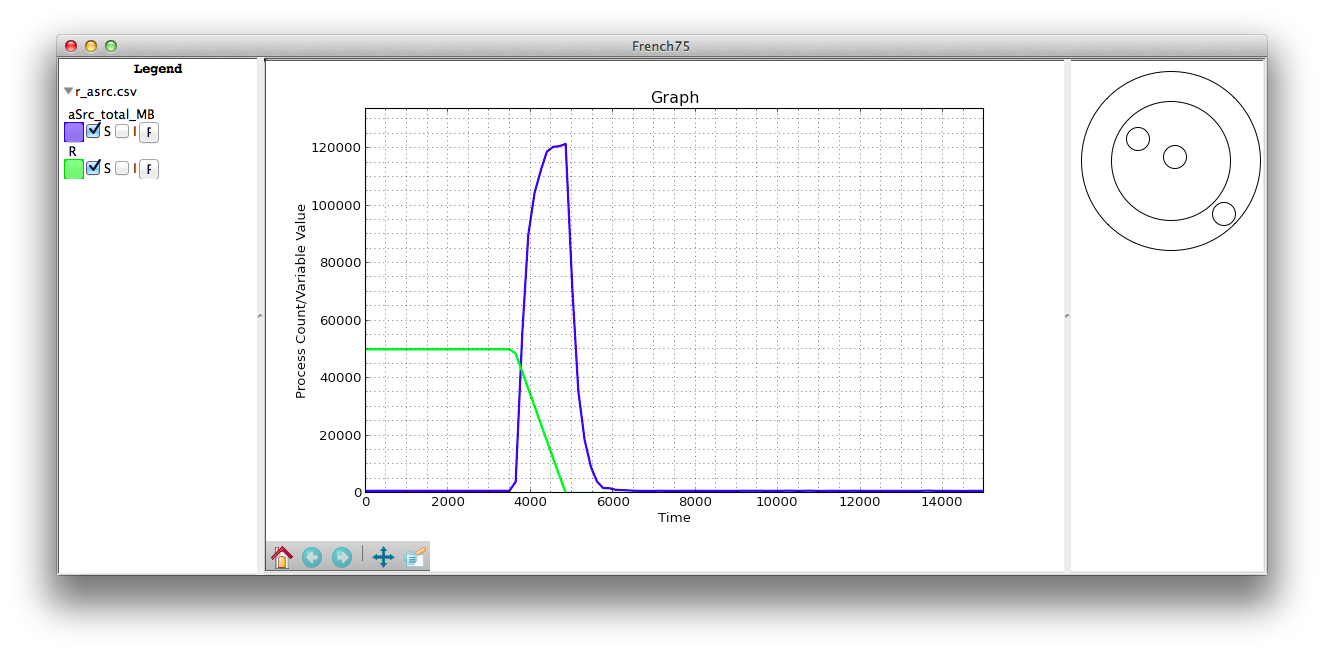
\includegraphics[width=\textwidth]{images/french75_mac.png}
    \caption{Main Screen of the Tool}
    \label{fig:f75_mac_intro}
\end{figure}

Over the course of the first stage of work a number of evaluations were carried out with potential and actual users of Bio-PEPA.  The findings from these evaluations were used to improve the tool.

\subsection{Results}

Break down by project stage?  Aniticipating this to be 1.5 - 2 pages


\chapter{Goals}
\label{chap:goals}

To help guide development during the project a number of goals were identified.  Over the course of the project the goals have been refined, new goals have been added and some goals have been dropped.

\section{Previous Goals}
Through research into the problem a number of goals were identified.  After performing a review of the existing software, the goals were refined.  The initial user evaluations also fed into the refinement of the goals of the project.  Some of these goals were completed in the first stage of development, the other goals were carried forward into the second phase of development.

The goals that were completed in the first stage of development are:

\begin{itemize}
\item Improve existing capabilities -- The purpose of this goal was to add to Bio-PEPA's visualisation capabilities and bring these more into line with the other modelling software.  This goal was completed in the first phase of development. The user was given extra control over the appearance of their graphs.  Intensity plotting was also implemented.
\item Visualise the model more intuitively -- The purpose of this goal was to help the biologists to increase their understanding of what the model and the graph is showing them.  This goal was completed in the first phase of development with the implementation of the hierarchical drawing of the model components.
\end{itemize}

The following goals were to be completed during the second phase of development:

\begin{itemize}
\item Provide visualisations that take into account the domain -- The purpose of this goal was also to help the biologists further understand what the model and the graph are showing them. This has been implemented in the second phase of the project.  This goal was merged with animation of the data.
\item Animation of the data -- The purpose of this goal was to make it easier for the biologists to interpret spatial data by showing the species in their results moving through the cell.  This has been implemented: the user can now visualise species moving through a cell.
\item Investigating which visualisation combinations work best -- The purpose of this goal was to try and work out whether there were any combinations of visualisations that the program could offer that the biologists found particularly useful.  This was originally planned to be performed in the second stage of the project, but due to the project focusing on non visualisation features the goal has been removed.
\item Add the ability to annotate the visualisations -- The purpose of this goal is to allow the biologists to add extra supporting information directly onto the visualisation. This goal has been implemented: the user can add annotations to the visualisations.
\item Allow the ability to save and load the program state -- The purpose of this goal was to allow the biologists to complete their work in multiple sessions. This goal has been implemented: users can save and load the program state into files, these can then be emailed to other users who can modify them.
\item Provide a full session history to the user -- The purpose of this goal is to allow the biologists to recover from any mistakes they might make. This has been implemented: the user has a full undo and redo history within the session allowing them to easily correct mistakes.
\item Data Mining -- The purpose of this goal was to have the program provide some level of automatic annotation and setting optimisation to reduce the workload for the biologists.  Due to other features being added that reduce the need for this goal, the goal has now been dropped.  The research for this goal was not lost however as a similar goal was added.  Data mining to identify features in not a goal that should be abandoned either, instead it would be implemented if the development continued.
\item Making meta data accessible -- The purpose of this goal was to display the experiment settings in the \ac{UI}.  This goal has not been completed in this phase of development.  It was pushed back to allow development on real time collaboration and plots as queries features.  It has not been abandoned, instead it would be completed if development was to continue.
\end{itemize}

\section{New Goals}
During the first half of the second phase of development new goals were identified.

\subsection{Data Manipulation and Export}

This goal was added after a meeting with the maintainer of BioDARE~\cite{biodare}.  This web based tool is aimed at results from laboratory experiments, specifically experiments relating to circadian rhythm.

BioDARE is an online biological data repository.  It allows its users to upload their experiment data.  This is then available to all other users.  BioDARE will generate static graphs of the uploaded data.  These plots have little ability to be customized.  Instead users can download the data and customize it in a separate application.

The maintainer explained that he had found that researchers often visualise their data after it has been normalised.  This removes any issues where different species have different scales and makes it easier for the users to interpret the data.

BioDARE can also export the raw data allowing the researchers to use it in other applications if they desire.

This seemed like a very useful feature for users and it was added as a project goal.

\subsection{Time Series Data as a Query}

There has been a lot of research in recent years~\cite{goldin, chakrabarti, popivanov, faloutsos2, bollobas} into using time series data as a query against a database of other time series plots through some similarity measure.

This would be a very useful feature to add to the tool.  By allowing researchers to use a plot as a query they would be able to discover other plots exhibiting similar behaviour.  This could be the same species reacting the same to different species, or a species that is exhibiting similar behaviour.  This could help the biologists discover alternative candidate species for research.

This feature would be most effective if there was an online repository of plots for the biologist to search.  This would also allow them to discover potential collaborators.  Online repositories of data do exist: BioDARE is one of them.  These repositories are unlikely, at the moment, to store the data in a suitable way to allow for efficient search.

Given the potential usefulness of this feature, and the fact that none of the other modelling software had this capability it has been added as a goal.

\subsection{Real Time Collaboration}

An important area where all the reviewed software were lacking is collaboration, real time or not.  The current work flow using the existing software is: perform your analysis, save it, email it to a colleague with additional files and notes and have them open it. They then attempt to work out the visualisation is showing.  It is a disjointed conversation.

It is not just the modelling software that did not offer collaboration. None of the visualisation software reviewed offered real time collaboration either.

Incorporating real time collaboration was added as a goal to offer researchers a better work flow.

\chapter{Work Done}

This section details the development work that has been performed in the second phrase of the project.  This includes conceptual problems faced, effectiveness of the result and any future work that could be performed.

%For each of the below, why, how inc conceptual problems, impact, how it could be improved

\section{Annotation}

Annotation was an important feature to add.  It is one of Grinstein's features that data visualisation software should have~\cite{gg_vizbi}.  This is because the purpose of a visualisation is to aid analysis.  If you have a print out of a visualisation you are able draw on it and highlight areas of interest.  Users need to be able to do this on digital versions of their visualisations.  As well as helping users analyse their data, being able to annotate also means that images for presentations can be prepared without having to save the visualisation and open it in an external program.  If you did this and then wanted to change the visualisation you would have to re-annotate it.  This is frustrating for a user and wastes their time.  Being able to do it from within the visualisation solves this problem as the raw data and the annotation data are together.  Another benefit of being able to annotate is having another way of attaching additional information to the visualisation when sending it to a colleague. Having this information on the visualisation saves them from flicking back and forth from an email or other supporting documentation.

Implementing annotation of the visualisations on offer in this tool had to be done in two parts.  This is because there are two parts to the annotation.  The graph and the cell level view.  One is a static visualisation and one is a dynamic visualisation.  Each of these required a different approach.  These are detailed below.

\subsection{Annotation of the Graph}

Annotation on the graph was relatively straightforward to implement.  matplotlib provides annotation capabilities in two forms.  One form is annotations that use arrows with or without text, and the other is arbitrary drawing on the graph.  Both of these forms have been utilised for annotations.

Users of the new tool are provided with four annotation types: arrow, text, arrow with text and circles.  Buttons for each of these annotation types have been placed on the matplotlib toolbar.  This can be seen in Figure~\ref{fig:annotation_demo}

\begin{figure}[h!]
    \centering
    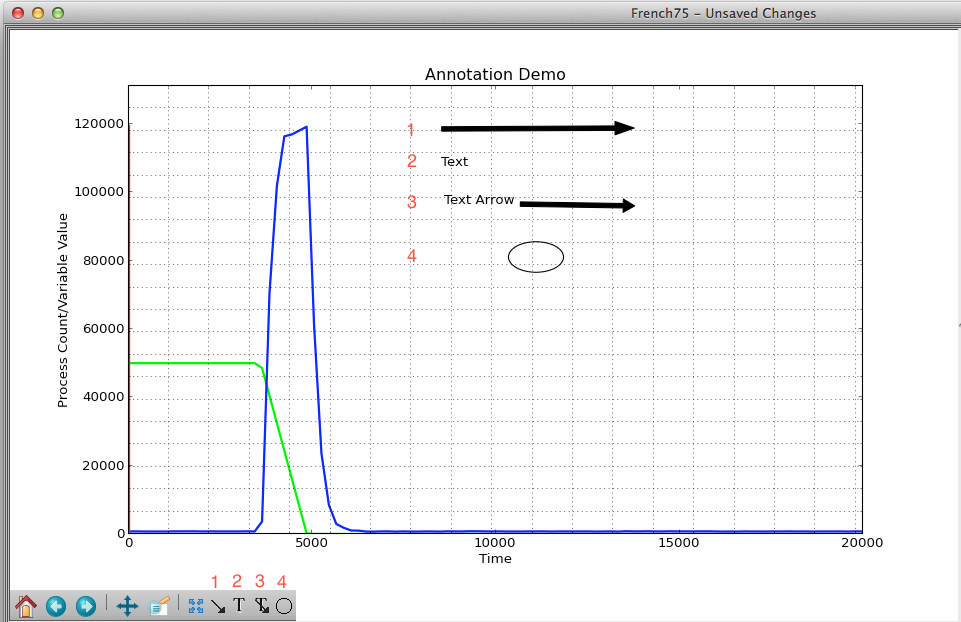
\includegraphics[width=\textwidth]{images/annotation_demo.png}
    \caption{Example of Each of the Four Annotation Types and the Toolbar Buttons that Correspond to Them}
    \label{fig:annotation_demo}
\end{figure}

There were problems in making the annotation creation process user friendly.  For all of the annotations the user needs to first press the appropriate button on the on the toolbar.  The next actions depend on the annotation type.  Text and circle annotations were intuitive as all they require is one click.  The user clicks where they want the annotation to be placed and it will be drawn on the graph there.  However the two arrow annotation types required two clicks.  The first click marks the start point (the tail of the arrow) and the second click is the finish point (the head of the arrow).  This was not obvious, when handed over to the users they didn't know that it required two clicks and didn't know whether the arrows would be drawn head to tail or tail to head.  The technique for placing arrows was changed so that the first click still fixed the position of the tail of the arrow. However the behaviour after the first click has changed, now a temporary annotation is continuously redrawn that has the head of the arrow wherever the mouse is.  This allows the user to see the arrow they are drawing.  To indicate to the user that they need to click on the graph the cursor is changed after pressing one of the annotation buttons on the toolbar.  The use of different cursors is a common technique to help guide users to perform actions.

It was important that annotations could be edited or deleted.  The annotations can not just be clicked as they are not a \ac{UI} widget like a button.  The solution to this was to have an array of annotations.  When a user right clicks on the graph it searches through all annotations and selects the annotation that was closest to the click (if that distance was below a certain threshold).  The selected annotation is then highlighted red, and a context menu appears to give feedback to the user that they have successfully selected an annotation.  This can be seen in Figure~\ref{fig:annotation_selection}  The context menu then gives the user the option to edit or delete an annotation.  Editing an annotation only allows for editing text.  For changing position the annotation has to be deleted and redrawn.

\begin{figure}[h!]
    \centering
    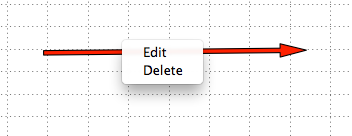
\includegraphics[width=\textwidth]{images/annotation_selection.png}
    \caption{Context Menu on Selection of Annotation}
    \label{fig:annotation_selection}
\end{figure}

To calculate the distance from the location of the mouse click to the annotation two problems had to be solved.  The first was how to calculate the distance from a point to a line.  An equation for this can be seen in Figure~\ref{fig:point_to_line_eq}.  Equation~\ref{eq:line} is the equation for a line in two dimensions.  This represents the annotation.  The equation can be calculated from the start and end points of the annotation. Equation~\ref{eq:point} is the position of the mouse click.  Equation~\ref{eq:distance} shows the equation for calculating the distance from the point to the line.  The second problem that had to be overcome was the difference in scale.  In effect we have two coordinate systems.  The results coordinate system and the visual coordinate system.  These difference are illustrated in Figure~\ref{fig:distance_scale}.  The annotations in Figure~\ref{fig:distance_scale_a} are further away from each other in the results coordinate system than the annotations in Figure~\ref{fig:distance_scale_b}, however they are closer in the visual coordinate system.  When selecting an annotation the user is using the visual coordinate system but the distance is calculated using the result coordinate space.  This could lead to the wrong annotation being selected.  The solution to this was to transfer one coordinate system into the other.  When calculating the distance from the point to the line the values are scaled by the size of the graph.

\begin{figure}[h!]
    \centering

    \begin{subfigure}[b]{\textwidth}
        \centering
        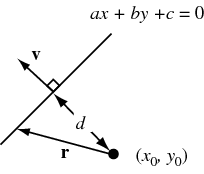
\includegraphics[width=0.3\textwidth]{images/point_to_line.png}
        \caption{Diagram of the Point to Line Distance Problem}
        \label{fig:point_to_line_diagram}
    \end{subfigure}

    \begin{subfigure}[b]{\textwidth}
        \begin{subequations}
            \begin{align}
            & y = -\frac{a}{b}x - \frac{c}{b} \label{eq:line}\\
            & (x_{0}, y_{0}) \label{eq:point} \\
            & d = \frac{\mid ax_{0} + by_{0} + c \mid}{\sqrt{a^{2} + b^{2}}} \label{eq:distance}
            \end{align}
        \end{subequations}
        \caption{Equations for Calculating the Distance From a Point to a Line.}
        \label{fig:point_to_line_equations}
    \end{subfigure}
    \caption{Equations and Diagram for Calculating the Distance From a Point to a Line (taken from WolframMathWorld~\cite{point_to_line})}
    \label{fig:point_to_line_eq}
\end{figure}

\begin{figure}[h!]
    \centering
    \begin{subfigure}[b]{0.6\textwidth}
        \centering
        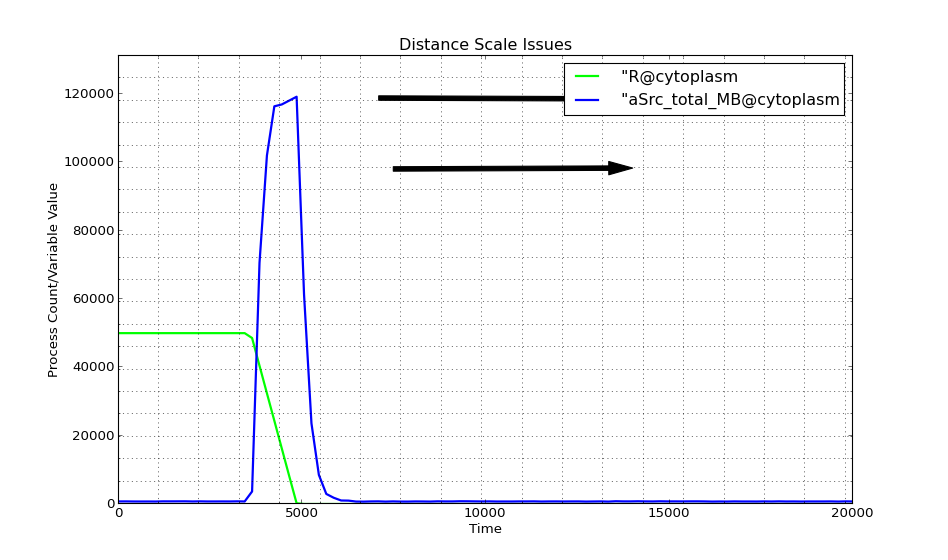
\includegraphics[width=\textwidth]{images/distance_scale_a.png}
        \caption{Annotations With Distance of Approximately 20000}
        \label{fig:distance_scale_a}
    \end{subfigure}

    \begin{subfigure}[b]{0.6\textwidth}
        \centering
        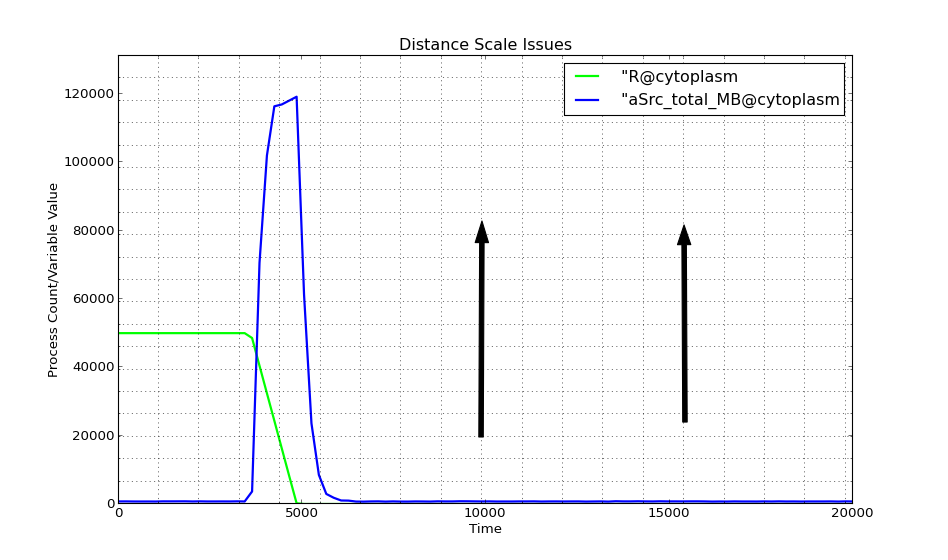
\includegraphics[width=\textwidth]{images/distance_scale_b.png}
        \caption{Annotations With Distance of Approximately 5000}
        \label{fig:distance_scale_b}
    \end{subfigure}
    \caption{Two Sets of Annotations Illustrating the Problems When Calculating Distance to an Annotation}
    \label{fig:distance_scale}
\end{figure}

A similar issue to the difference in scale when calculating the distance from the mouse to annotation was encountered when switching the graph to normalised mode.  When normalised the graph in the y axis only goes between 0 and 1.  The coordinates of the annotation are likely to be very much outside this range and the annotation would not appear on the graph.  The solution was to if the graph is normalised then to also normalise the positions of the annotations when drawing them.  A side effect of this technique is that the lines are potentially going to rescale themselves.  This could leave an annotation point to nothing.  This is unavoidable as the annotation has no concept of what it is pointing at.  It may be pointing to the intersection of more than one line, in this case it would be impossible to keep the annotation pointing at what it was originally pointing at.  Neither of these is optimal.  Both approaches lose the information that the user originally added.  During user evaluations, when the annotation would not be visible during data normalisation, the user was very confused as to why their annotation had disappeared.  It was therefore decided to have the annotation be visible but most likely incorrect as it is clearer to the user what has happened.

\begin{figure}[h!]
    \centering
    \begin{subfigure}[b]{0.6\textwidth}
        \centering
        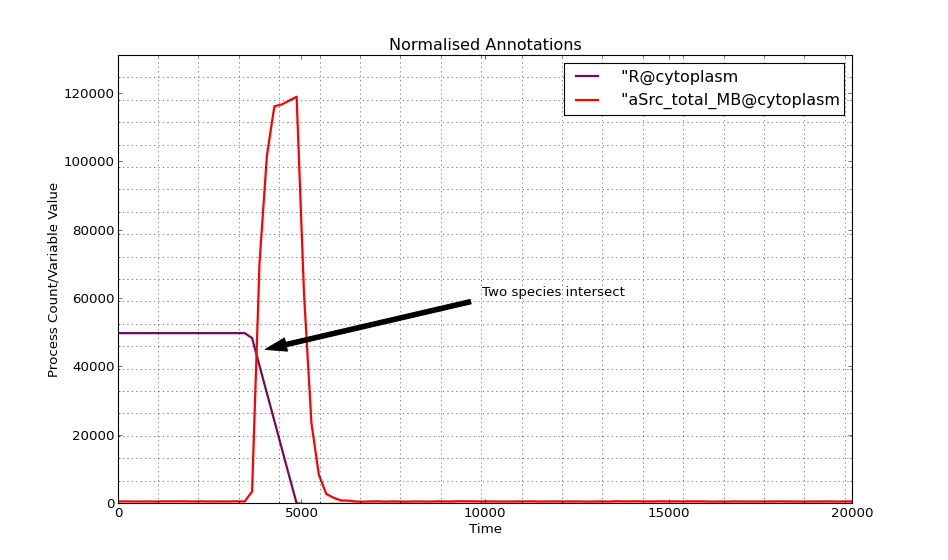
\includegraphics[width=\textwidth]{images/unnormalised_annotation.png}
        \caption{Annotation Pointing at Correct Intersection of Species}
        \label{fig:distance_scale_a}
    \end{subfigure}

    \begin{subfigure}[b]{0.6\textwidth}
        \centering
        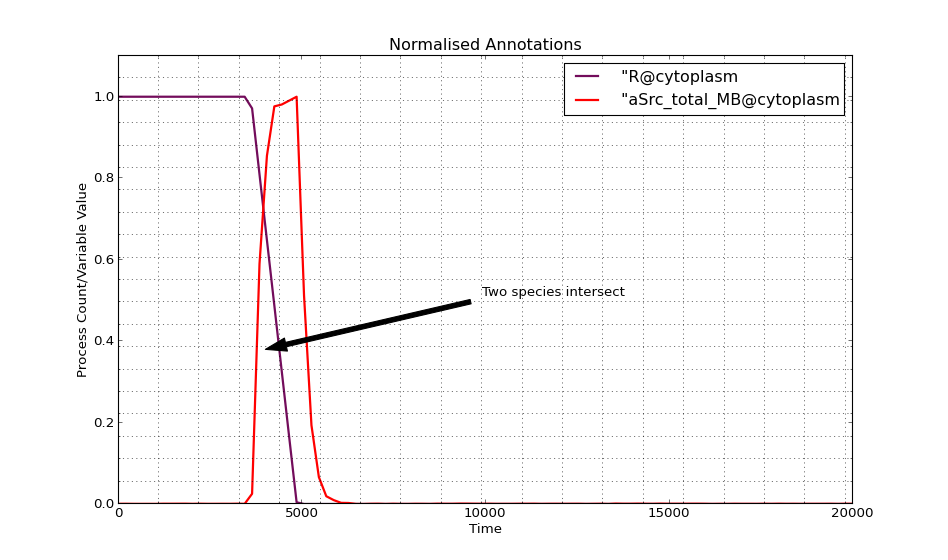
\includegraphics[width=\textwidth]{images/normalised_annotation.png}
        \caption{Annotation Pointing at Nothing After Data Normalisation}
        \label{fig:distance_scale_b}
    \end{subfigure}
    \caption{Graphs Illustrating What Happens to Annotations Whilst Data is Normalised}
    \label{fig:distance_scale}
\end{figure}

\subsection{Annotation of the Animation}

After completing annotation of the graph it was important to expand this to the animation panel, as this is the other area where visualisations are put.  This posed more of a challenge than for annotation of the graph and there were a number of issues to overcome.

\begin{enumerate}
\item How to implement the annotations?  For the graph matplotlib has built in annotation support.  wxPython does have drawing support but not in built annotation support.  Annotating on the animation will need manual handling of the drawing on top of the animation visualisation.  Manual drawing means that the automatic layout functionality that wxPython provides cannot be used.
\item When to display the annotations?  When an annotation is drawn on the graph it is displayed at all times.  The appearance of the graph does not change over time.  However the appearance of the animation visualisation does change over time.  The problem faced when annotating is whether to have annotations available at only specific times in the animation, or to have them there the whole time, and if they are going to appear and disappear how can it be done without being distracting?
\item How to give the user control over the annotations? When a user wants to edit or delete an annotation on the graph it is always there.  However on the animation panel if the annotation is temporal, then it is not always visible for the user to edit or delete and it would be frustrating for a user to constantly have to search through the animation to look for annotations to change them.
\end{enumerate}

\section{Animation}

THIS NEEDS A LOT OF WORK

Animation was a key goal of the project.  The core aim of the project is to help biologists who aren't comfortable with traditional time-series graphs.  So the goal was to provide them with visualisations closer to what they see in their domain.  This has been accomplished by displaying spatial data in the shape of the cell.

The animation is ideally used to display species moving through a cell.  This collapses what would be multiple different lines in a graph, that give no indication of their real position in the cell, into a single image.  There is one segment in the cell animation for each line.  The colours in each segment reflect the colour of the line on the graph.  Then over the course of the animation the colours are set by the colour in the intensity plot version of the line.  This allows the researcher to compare the two visualisations and will hopefully help build their confidence on the graph plot.

To make setting up the animation user friendly to control required the model file so that the location hierarchy could be parsed.  Before this there was an awkward system where the user had to input where in the cell a species is.  This was time consuming, awkward and quite brittle.  At the time it assumed that there would be three compartments in the species, which is a terrible assumption to make.

The requirement of the model file for parsing animation has also led to animation replacing the previous model visualisation.  In the set up phase after the the model and the species have been parsed the user is presented with a cell segment, similar to what is seen in the animation panel.  The cell segment is split into different regions, one for each region of the cell.  These segments are then coloured if the selected species is present in them.  The user can select between all species in the selected results files.  This has a number of benefits.  First, they can sanity check that they have matching results and model files.  Second, they can see how the model is structured.

Similar control is provided on the animation panel itself.  The user can see the animation focused on a specific species, in which case a cell segment is drawn for each file that the species is in.  Or they can have the animation focused on a specific results file in which case a cell segment is drawn for each species in that results file.

\section{Data Mining}

\section{Search}

Using a time series as a plot posed some interesting problems.
\begin{itemize}
\item How to cope with different scales
\item How to cope with events happening at different times
\item How to represent the plot to allow for efficient search
\item How to determine similarity between two graphs
\end{itemize}

All of these needed to be overcome for this feature to be useful.

This is an area of active research.  Early techniques used simple techniques such as Euclidean distance, but these simple approaches gave poor results.  It is feasible to have a species that exhibits a similar reaction to our query (the line has the same shape) but it happens at a different time in the experiment than our query plot.  In other words the graph is offset.  We can tell that the two graphs are similar, but euclidean distance will return that they are unsimilar.  The same problem occurs with differences in species population giving an offset in the x axis.

After researching current techniques an approach was taken that solves all the problems above.

The first step is to convert the input data to be a list of all n length sub lists of the input data. i.e. with input data [1,2,3,4,5] and n = 3 our input data would become [[1,2,3], [2,3,4], [3,4,5]].  The sub lists are our features.  We then normalise each feature to be zero mean, unit variance.

The next step is to convert the continuous data into discrete data and reduce the dimensionality of it.  By normalising the data to be zero mean and unit variance we have allowed a normal distribution to be easily fitted to our data.   Using the normal distribution we convert a data point in our sub list to be one of three possible values.  Here we use the characters `a', `b' \& `c'.  This builds a string representation of the plot.

The paper this approach is taken from then calls for reducing local duplicates.  This further reduces the size of our fingerprint and increases the efficiency.  Removing the local duplicates means any ignoring runs of a certain string can be replaced with just one instance of the string.

This provides us with a finger print of the plot.  A string size of 8, with 3 possible value leads to a vocabulary size of 6561 possible representations.  A single plot will have very few of these, so we use a sparse representation.  For each line a dictionary is stored.  The dictionary keys are the strings in the fingerprints and the value is the count of that string in the plot's fingerprint.

This format of the fingerprint also solves the problem of similar features happening at different times.  The plot fingerprint is a bag-of-words, in this case a bag-of-features.  There is no order to them, it is as though we are assuming that all features appear at the same instant.

Now that we have a representation of the plot that is scale and time invariant and allows for efficient comparisons we can find a method to calculate the similarity.

We could simply just use Euclidean distance again, but this does not do anything to weight rarer features that can tell us more about a graph.  An alternative distance measure would be cosine distance, but this suffers the same drawback.

It was decided to implement tf.idf weighted cosine as the similarity measure.  This takes into account term frequencies to provide a higher weight to rarer vectors.  tf.idf is very well researched in the field of information retrieval and text mining.  Given the representation of the finger print is equivalent to a bag-of-words it seems sensible to apply tf.idf to this domain.

\subsection{tf.idf} is a way of ranking how important a word is.  Taken into account are frequency of a word in the query, frequency of a word in the document, length of the document, average length of documents in the corpus, total number of documents and frequency of the word across all documents.

The formula is: INSERT FORMULA.

These term weights are then used in a tf.idf weighted cosine.

This approach allows for effiecient search.  If we have two indexes.  One where keys are the documents and the values are the words in the document and their frequencies. Then we have another index, an inverted one.  Where the keys are the words and the values are a list of documents that contain them.  The individual components of the tf.idf equation can therefore be calculated with very little effort.  This means that a plot can be compared to the database of plots in O(n) time.

Initial results are very promising with the tf.idf weighted cosine providing much clearer results than with simple euclidean distance.  There is not a large enough truth set of plot similarities to be able to confidently say that it is effective.  However these early promising results seem to indicate that further research would certainly be worthwhile, but outside the scope of the project.

DISCUSSION OF THE EARLY RESULTS

\section{Collaboration}

The initial step of allowing collaboration is enabling two instances of the program to talk to each other.  There are a number of techniques to allow for this.  Data could have been sent directly through sockets, another option would be to create a web server and send get requests and pass parameters.  It was decided to use an existing library to handle the communication.  The library chose was simplexmlrpc.  This allows each instance to run a client and a server.  The server has an api and this can be called.

On initial connection the `master' sends its entire session state the the `slave' uses this as its initial state.  After this whenever either client performs an action it issues a call to the other clients server to perform the same action.

An issue that was encountered is how to ensure that both clients are seeing everything in the same order.  Lamport clock proved to be the solution.

\section{Usability}

In all the evaluations of the project users have commented on the difficulty of using parts of the tool.  Action has been taken to make it easier to use.  Many of the changes have been guided by Shneiderman, Norman \& Nielson's guidelines.  Specifics are detailed below.

\subsection{Undo \& Redo}
Shneiderman calls for easy reversal of actions and Nielson calls for user control and freedom -- an emergency exit from an unwanted state.  To address this, an undo/redo functionality has been added.  This required refactoring of the project code, so that the session data is in one location, inside a singleton. Any changes to this data are picked up during the next \ac{UI} update and are reflected in the visualisations.  The session data is stored as a dictionary.  To implement undo and redo, copies of the data dictionary are pushed and popped onto the stack.  Copies are pushed onto the undo stack on any atomic change the user makes.  This gives the user a full session history to go back through and this was one of the early goals from the first project phase.

A problem was encountered when trying to copy the dictionary onto the stack.  When just pushing the dictionary onto the stack it would not put a new copy of it onto the stack, so any changes to the dictionary after it has pushed onto the stack are also there in the stack.  Python dictionaries have a copy method.  Copy only does a shallow copy -- any objects in the original dictionary will have their reference placed in the new dictionary.  This was fine for some parts of the session dictionary, but for others it was not. In particular, lines and annotations, which are custom objects presented problems.  This was solved by using deep copy.  With deep copy a new copy is made of objects as well.  Some elements of wxPython and matplotlib were unable to be deep copied, but this was fixed whilst focusing more around the data -- so the \ac{UI} elements use the data, not the other way around.

\subsection{Saving}

It is important that a user is able to save and load the visualisation session as they may not be able to complete all their analysis in one sitting and may want to come back to their work in the future.  Without the ability to save and load the user would have to repeatedly add annotations and change preferences and attach files.  It was possible to add Saving and loadingby building on the work done to implement undo \& redo, although further work was required. Python has a module called pickle to serialise and deserialise data.  When saving, the dictionary containing the session data is pickled and written to a file and when loading the reverse happens.  Because the program is now focused on the data model, once a previous session has been loaded, a \ac{UI} refresh is triggered and the visualisation reflects the loaded data.

Saving the data also enables limited collaboration.  The user can customize the appearance and add annotations.  They can then save the state to a file and email that file to a colleague.  The colleague can then load the file and see the user's work.  The colleague can then correct any issues and add their own work.  The colleague can then save this and email it back to the user.  This is useful and is better than no collaboration, but it is entirely non realtime.

\subsection{Feedback}
Norman and Shneiderman both call for feedback to be given to the user so that the user can be sure that an action has been accomplished.  This feedback can come in a number of different forms and was in place in some parts of the project already.

Existing feedback in the project was a natural byproduct of some of the features; for example, when loading a results file the feedback that the load operation has been successful is that a graph appears on the screen. If the graph does not appear then something has gone wrong.  Additional feedback has been added to the project:
\begin{itemize}
\item When adding annotations the cursor changes to indicate to the user that they can interact with the graph in a different way.
\item The title bar text changes to display ``unsaved'' when the user makes a change and then changes back to ``saved'' when a successful save has been performed.
\end{itemize}

\subsection{Guiding the User}

The first evaluation of the second phase of the project unearthed that the users struggled to choose the correct action as there were multiple ways of doing the same action that had slightly different use cases.  There was also confusing language in the menu options.  These multiple paths have been removed. For example, now there is only one way to open results files initially.  To help guide the user further \ac{UI} elements are enabled and disabled as appropriate.  Now when the program is first loaded the only action a user can perform is to load a session or start a new session.  Afterwards other \ac{UI} elements are enabled to allow the user to start using the tool effectively.

\section{Data Manipulation and Export}

\section{Finished Product}
Overview and walkthrough of tool

\chapter{Evaluation}
\label{chap:eval}

This section relates to the evaluation of various aspects of the project.  The Src researcher whom the project focused around was off on maternity leave for the duration of this phase of the project so no evaluations were able to be performed with them.

\section{First Evaluation}

The first evaluation in the second phase of the project occurred in November 2013.  The user group was made up of two biologists.  One who had taken part in the first evaluation meeting and one person who had no knowledge of the project.

\subsection{User Group}

As the domain expert was not available, insight based evaluation was unable to be used.  A more traditional approach had to be taken.  Before the evaluation  a typical scenario that a user might encounter was prepared.  The task was to open a file, annotate it and run the animation visualisation, and attach supporting documentation.  The task was prepared at two levels of instruction.  The first level was a paragraph of text that described what was to be done.  The second level was a step-by-step list of instructions to perform.  The user group was observed as they attempted the task and were offered assistance when required.  Afterwards the user group was given a questionnaire to fill in about their experience. After filling in the questionnaire there was a discussion on their answers and any further thoughts that they had.

The task was prepared at two levels to try and gauge how easy the program is to use.  The users were first presented with the textual description and if they had been unable to complete the task with this then they would have been given the step-by-step instructions instead.  The users were able to complete the task from the textual description alone.  This is a good sign that the new tool is usable.

Some issues were encountered:

\begin{itemize}
\item The users were unfamiliar with MacOS -- Both users were unable to locate the menu bar as it is not attached to the program as in Windows.  Future evaluations will use Windows.
\item The users were unclear as to what was going to happen when annotating.  When annotating the graph with an arrow the user had to click twice to place it but there was no indication of this, nor was it clear to them which way the arrow would be drawn.  This has now been fixed. Different cursors are used to give feedback to the user that they should click, and rather than just relying on two clicks with no information as to where the arrow is going to point, after the first click (which places the tail of the arrow) an arrow will be drawn that follows the cursor until the second click placing the annotation.
\item Lack of ability to edit, move, or delete annotations -- Once an annotation was placed it was there permanently.  The ability to edit annotations was always planned, but had not been implemented in time.  But the amount of frustration it gave the users was very high.  It was a principle in all three of Norman~\cite{normsev}, Neilson~\cite{neilten} and Schniederman's~\cite{shgold} lists that a user should be able to fix mistakes.  Since the evaluation, editing and deleting of annotations has been implemented.  This means any mistakes can be corrected.
\item Initially the users were confused by what all the buttons on the matplotlib toolbar did.  After discovering the tooltips, and seeing what effect the buttons had, they were comfortable with them.  If a user were to do something they did not intend they are able to undo it. All the matplotlib built-in buttons on the toolbar can be undone and redone from the toolbar.  Any buttons implemented for this tool are covered by the undo and redo functionality implemented across the whole program.  Being able to recover from their actions on the toolbar means no hindrance to discovery and so needs no further action.  It would be desirable to have the two undo methods unified but a way to do this could not be found.
\item The users were confused by some of the terminology.  In particular the could not distinguish between ``save graph'' and ``save model''. These items in the menu have now been grouped more carefully to help the user distinguish them.  A related issue was worrying that ``save graph'' was going to override the results file.  To rectify this the menu items that create new files have been renamed ``export ...''.
\item The users struggled to start a new session.  When asked for a title they did not know what the title was going to be used for.  When trying to add files, rather than use the add files button in the dialogue, they tried to use the file menu.  Having two routes into the visualisation seemed to be confusing them.  Now the file menu open file has been removed.  To create a visualisation the user has to go through the new session wizard.
\item When placing species in the cell one of the users did not understand what they were being asked to do.  One of the users did understand.  To fix this user input has been removed from the process.  The species locations are parsed automatically from the model.  This has required the model file to be added to the session by the user.
\item They liked the animation feature and thought it would be very useful (One of the users did their PhD in transport and expressed a desire to have had this feature during the PhD).  They did feel that it wouldn't be useful directly for papers, but that it would be useful when deciding what to include in a paper.
\item One of the users asked if there was a map of the cell.  When presented with the model visualisation they thought that it did look nice, but they were unsure of its usefulness.  The model viewing has since been merged into the animation visualisation.
\item The results from the questionnaire indicated that both users thought the tool's appearance was good.  The tool was average in difficulty to use -- neither easy nor difficult. The annotation buttons on the toolbar were clear as to what they did. It was obvious how to attach supporting files.  Both users thought that it is very useful to attach files to the session so that they can be easily emailed to a colleague.  They thought it would be useful to have the graph automatically annotated, but they wanted to the ability to disable any automatic annotations.  Both users found the animation useful.
\end{itemize}

\subsection{Personal}

At this stage in the development the program was in a state where some existing functionality had been broken.  This had not been noticed during development.  This highlighted architectural flaws in the code.  There were multiple paths through the program that data was taking.  Code was also duplicated across the program.  Since then a majority of these bugs have been ironed out and the duplications removed. The code is now better architected.  At the time of the evaluation with the users not all the features could be tested with them -- mainly the plot preferences dialogue.  These features have now been fixed and they will be evaluated by the users at the next meeting.

Having the users use the program has also highlighted a number of usability problems: menus being badly organised and named, features such as annotation rely on assumed knowledge to work them.  All this created an unfriendly environment for the user.  This was due to losing sight of the need for usability during development and when testing new features not removing the knowledge of the code from my mind.  Since this evaluation the three lists of usability~\cite{shgold}\cite{normeval}\cite{neilten} have been refocused on and the code gone through and the principles applied.

The positive feedback on animation and annotation, two of the core new features, is excellent validation of the new work.

\section{Evaluation 2 - Start of Second Semester}

The second evaluation in the second phase of the project occurred in February 2014.  There were two evaluations this time.  One with the same group of biologists as before and another with an Informatics researcher who uses Bio-PEPA.

Since the last evaluation work had been done to fix the issues encountered since the last time and two new features had been added: annotation of the animation and data normalisation and export.

\subsection{User Group}

As with the first evaluation a task was prepared at two levels of instruction.  Afterwords the users were given a questionnaire to fill in.  They were also given a chance to use the program without following a task, giving them a chance to explore.  Again, after the questionnaire a discussion was held.

The findings of the evaluation were as follows:

\begin{itemize}
\item There were inconsistencies in the text giving instructions to the user.  This did not appear to cause confusion, but it was noticed by both of the users.  This was fixed.  All the user facing text in the project was checked and changed if necessary.
\item The users kept trying to drag annotations on the graph after creation. The users wanted to be able to drag the annotation to a new position to fine-tune the position.  They attempted to do this by left clicking on the annotation and dragging it.  This issue has not been solved.  Currently if the user places an annotation in the wrong location they can delete the annotation and put a new one in the correct place.  For the user this is not the most desirable solution, but it was felt that the time could be better spent in other areas of the project.  This would, hopefully, be implemented in future work.
\item The users found the new model visualisation much more informative.  This is a positive as the reason for implementing model visualisation was to help the users understand what happens in the model more.  The users did however think that adding in labels of the compartments would be useful as they may not be familiar with the model.  The labelling of compartments has since been implemented.
\item The users found the task to be easy to complete.  This is a good result.  The tool needs to be easy to use.  They did not give full marks for ease, so there is still room for improvement.
\item The users found it much easier to start a new session using the wizard.  This was a task they had struggled with during the previous evaluations.  There were still aspects that they did not discover such as being able to select multiple files.  Guidance text has since been added to the wizard pages.
\item The users indicated that they found annotating animations easy and intuitive.  This is positive.  It is a new feature and the users indicated little need for change.
\item The users uncovered some bugs in the system.  The bugs included: not all types of annotations being able to be placed on the plot and the colours of the cell segments not being updated after changing the colour of the line.  All bugs discovered have since been fixed.
\item The users were very much in favour of being able to use plots as queries.  This provided justification for pursuing it as a project goal.
\item The users were very much in favour of being able to collaborate in real time. This provided justification for pursuing it as a project goal.
\item The users found it easy to normalise \& export the data and indicated that they thought it would be a useful feature to have.
\item The users were pleased by the addition of undo functionality.  They appeared to be much more willing to make mistakes knowing that they could undo their mistakes.
\item The users were pleased that since the last evaluation the ability to modify and delete annotations had been added.
\end{itemize}

\subsection{Bio-PEPA Developer}

The evaluation with the Bio-PEPA developer was similar to the evaluation with the user group.  The developer was given the same task and after performing the task there was a discussion about their performance and their feelings about the tool.

\begin{itemize}
\item It was not clear to the user what the new model visualisation was displaying.  This has been solved by adding text to the model visualisation page explaining what the user is seeing.
\item The user uncovered a bug in how annotations are rendered when the graph is viewed with the data normalised.  The problem and the solution are discussed in Section~\ref{sec:annotation_graph}.
\end{itemize}

\subsection{Personal}

The results from this evaluation were positive.  The users seemed much more comfortable using the tool.  This was hopefully down to the efforts made to improve the usability.  There are still too many bugs being discovered by the users.  This was addressed by spending a significant amount of time on tracking down and fixing bugs.  The positive reception to the ideas for plots as queries and real time collaboration led to them being added as project goals.

\section{Evaluation 3 - End of Second Semester}

The third and final evaluation in the second phase of the project occurred in March 2014.  There were two evaluations this time.  These were the same as the previous evaluation: the user group and an Informatics researcher who uses Bio-PEPA.  Given that this was the final evaluation a further focus was placed on evaluating the users preferences between this new tool and the Eclipse plugin.

Since the previous evaluation a sizeable amount of work had gone into improving the stability.  The new features that had been added were plots as queries and real time collaboration.  These were unable to be evaluated by the users. Plots as queries could not be evaluated as it has not been tied into the \ac{UI}.  Real time collaboration could not be evaluated with the users as it would have required another laptop.  The layout of the program had changed and this was tested by the users.

\subsection{User Group}

Like the other evaluations the users were given a task to complete.  Afterwards there was a questionnaire and a discussion.

The findings are as follows:

\begin{itemize}
\item The users liked the appearance of the tool.  Since the previous evaluation significant effort had been placed into making the user interface more aesthetically pleasing.  The users strongly preferred the new \ac{UI}.  This justifies the effort into the \ac{UI}.
\item The users indicated that they found the task easy to complete.  They were not confused by the new layout.
\item Both users indicated that they would rather use this than the Eclipse plugin.  They did both give the proviso that they have zero experience with the Eclipse plugin beyond what they were shown in the evaluation.  In the evaluation they were shown an example of a graph the the plugin generated.  Both users being willing to use this new tool instead of the Eclipse plugin is excellent validation of the project aims.
\item Both users were unable to give feedback as to what features they felt were missing or features they would like to see as they had not spent enough time with the tool.  Further evaluation time with ethnographic studies would be required for this.
\item When creating an animation annotation the users set the duration to be after time zero.  They were confused afterwards as to why the annotation was not immediately visible on the cell.  It had been hoped that it would be obvious that if the current clock was not in the duration of the annotation that it would not be visible.  This was solved by updating the clock to be the start time of the annotation being created. This means it is always visible to the user that an annotation has been successfully placed.
\item The slowness of the tool caused the users some frustration.  They would frequently be wanting to perform the next action, but the program was still trying to update the visualisations.  This is a problem that has been discovered with matplotlib -- it is quite slow.  This has not been resolved.
\item The users found the model visualisation more helpful now that labels had been added.
\item The users appreciated the addition of helper text to various parts of the \ac{UI}.
\end{itemize}

\subsection{Bio-PEPA developer}

The user was presented with the same task as the user group.  After completing the task they were asked to fill in a questionnaire.  After filling in the questionnaire there was a discussion about their performance.

\begin{itemize}
\item The user felt that the appearance of the tool was adequate, although they far preferred the new \ac{UI}.  They did not rate the appearance as highly as the biologist users.  They were unable to explain why they had not scored it higher in appearance.  They said would like to see more headings on the different parts of the \ac{UI} in the future.  This would be resolved if development were to continue.
\item The user indicated that they found it difficult to complete the task.  In previous evaluations they did not find it as difficult.  This was due to the lag in the \ac{UI} when updating the visualisations.
\item When asked whether they would use this tool instead of the Eclipse plugin the user said it depended on what task they were trying to perform.  If they were preparing images for publication they would use this new tool.  If they were just analysing the model they would use the Eclipse plugin.  This was to be expected.  Future work would hopefully be done to integrate the workflow between the Eclipse plugin and this new tool.
\item The user would have liked to see the model visualisation being able to handle models that were not necessarily hierarchical.  This would hopefully be looked into for future work.
\item The user would have liked to have been able to evaluate the tool with more models which covered a variety of scenarios.  This was not possible in this evaluation strategy. A direction for future evaluations would be ethnographic studies.
\item The user did not discover the context menu for annotations, they had to be told of this.  No solution has been found to make this feature more discoverable.
\item The user uncovered an issue that made it very difficult to right click on text or circle annotations.  These annotation types use point to point Euclidean distance.  This meant that the user had to right click near the start point of the annotation.  This start point is not obvious at all.  This problem has not been fixed.  For the circle annotation it would be possible to use the equation of a circle to check if the mouse click is near any point in the circle.  For the text annotation it would be very difficult to solve as the text annotation has no concept of its size.
\end{itemize}

\subsection{Personal}

The final evaluation definitely revealed that project has had positive outcomes.  The user were all in favour of the project and would use it in their workflow.  The reception to the new \ac{UI} layout was very positive.  Fewer bugs were discovered than in previous evaluations. There are still usability flaws and further, more in depth evaluation is needed.

\section{Self Evaluation}
The feedback from potential users was a very important part of the evaluation.  There are other important aspects of the evaluation.  There are other metrics for what constitutes a good, usable piece of software.  The performance must be evaluated.  We must also consider the validity of any results.  These aspects, and more, are discussed in this section.


\subsection{Evaluation of the Architecture}

In Section~\ref{sec:architecture}, the architecture of the tool is discussed.  During the second phase of development the program was given an architecture similar to \ac{MVC} but with little distinction between the view and the controller.  This was a step in the right direction.  The program would, however, have a much better architecture if it was fully \ac{MVC}.  This would have the implementation of real time collaboration much easier. Having a \ac{MVC} architecture would also make future development easier.  This is discussed in Section~\ref{sec:conc_architect}.

The program architecture suffered towards the end of development when real time collaboration was added as a feature.  The code was not fully \ac{MVC} and collaboration had not been a potential feature during any the architectural design.  This feature introduced an entirely new route through the program.  Due to the project time table there was no time to refactor the architecture.  This led to collaboration being somewhat bolted on.  Some of the functionality necessary for real time collaboration was put into the singleton object.

\tdi{Does this contradict too much of what I said in the implementation chapter?}


\subsection{Meeting HCI Principles}

Norman~\cite{normsev}, Schneiderman~\cite{shgold} and Neilson~\cite{neilten} each have a set of principles for \ac{UI} design.  Whilst planning this project is was decided that these principles would form a useful evaluation metric.  The principles and how this project meets or does not meet them are detailed in the section.  There are overlaps between the sets of principles.  If there is an overlap it has been indicated.

\paragraph*{Striving for consistency} is a principle in all three lists.  It suggests that platform conventions should be followed, similar actions should have similar effects and terminology should not change across the \ac{UI}.  Conforming to platform conventions has not been strictly followed in this project.  The intention was to be cross platform.  An attempt was made, with respect to the menubar, to follow MacOS guidelines.  However there are not enough menu options to make this obvious.  Terminology has been kept as consistent as possible across the \ac{UI}.  Efforts were made for similar actions to elicit similar results, however this was not always successful.  There is a big inconsistency between built-in matplotlib functionality and functionality implemented by this tool.  For example there are two different undo mechanisms.

\paragraph*{Enabling shortcuts} is principle in Schneiderman's and Neilson's principles.  Shortcuts are there for expert users to save them time.  There are standard shortcuts, i.e. Ctrl-S for save.  Standard shortcuts can be considered user friendly.  Custom shortcuts are not user friendly, but they enable an experienced user to speed up their workflow.  Standard and custom shortcuts were implemented in this tool according to wxPython specification.

\paragraph*{Offering informative feedback} is in all three lists of principles.  This is so the user is kept aware of system state.  They should be receiving feedback from every action.  This is detailed in Section~\ref{sec:feedback}

\paragraph*{Designing dialogues to yield closure} is a principle in Shneiderman's principles.  It calls for encapsulating sequences of actions with dialogues.  Finishing the dialogues allows the user to clear their mind.  The new tool makes significant use of dialogues to improve the user experience.

\paragraph*{Offering simple error handling} is a principle of Shneiderman's and Neilson's principles.  The user should be prevented from arriving at an error state.  This was a problem throughout the project.  During development the found error states were removed, this was done through exception catching and more defensive programming.  If new error states were discovered the same techniques would be applied.  If the user performs and action they did not mean to, which could be classed as an error, they are able to undo it.

\paragraph*{Permitting easy reversal of actions} is a principle in Shneiderman's and Neilson's lists.  It is intended to give users a way of escaping error states by reverting to previously working states.  This has been implemented through undo and redo.  This is discussed in Section~\ref{sec:undo}.

\paragraph*{Supporting internal locus of control} is one of Shneiderman's principles.  It calls for making the user feel in control of the system and having the user instigate actions rather than respond to actions.  The user is the instigator of all actions in the tool.  The sense of control will be lost when collaborating as actions will be perform that they did not instigate.  This is unavoidable and is also mitigated by the fact that the users have to instigate a collaborative session.

\paragraph*{Reducing short-term memory load} is a principle in Schneiderman's and Neilson's lists.  It calls for keeping \acp{UI} simple.  It is important that users should be able to recognize what action needs to be performed, not remembering what action has to be performed.  This has been done by clearly and effectively labelling \ac{UI} elements and by having a shallow structure.  The user is not forced to go through deep menus and dialogues to perform actions.  When implementing recognisable \acp{UI} it is important not to end up in a Norman's door situation \tdi{Cite Norman's Doors}.  A Norman door is a door that has been particularly poorly designed and is labelled push or pull, rather than made clear through the design of the door, usually the handles.  Some minor Norman door situations have found their way into the project.  The most obvious one is in the session wizard on the results file selector page.  The user is able to select multiple files.  The user did not discover this, so helper text was added telling the user that multiple files can be selected.  It had been assumed to be obvious, as it is a feature in many programs that you can select multiple files.

\paragraph*{Constraining the user} is one of Norman's principles.  It suggests finding ways to restrict what actions a user can perform during use of the program.  This can be used to help guide the user through the program.  This has been accomplished in this project through the use of wizards and by enabling and disabling various \ac{UI} elements.  This is discussed further in Section~\ref{sec:guiding}

\paragraph*{Providing mappings to the real world} is one of Norman's and Neilson's principles.  It suggests that the program should `speak the user's language' and use words phrases and concepts that are familiar to them.  The cell cross-section animations are an example of that in this program.  It maps the results data into a form that is more familiar to biologists.

\paragraph*{Making use of affordances} is one of Norman's principles.  Is calls for using visual clues to help guide the user.  Different mouse cursors were used to indicate to the user that different functionality could be performed.  This is detailed further in Section~\ref{sec:guiding}.

\paragraph*{Having an aesthetic and minimalistic design} is one of Neilson's principles.  It calls for not having unnecessary in the \ac{UI} as it competes with the relevant information for the users attention.  This is quite a subjective criteria, however the user feedback would seem to indicate that it has been met.

\paragraph*{Providing help and documentation} is one of Neilson's principles.  It calls for having documentation be available for the user in case they need it.  This project has no user documentation.  This is because the time that could have spent writing documentation was better spent implementing innovative features.  If time was not a factor in the project then user documentation would have been written.

The new tool has been quite successful at meeting these principles.  We can consider therefore to be good interface, with room for improvement.

\subsection{Visualisation Quality}

Edward Tufte's The Visual Display of Quantitative Information~\cite{tufte} is a seminal work in the data visualisation field.  In this book he outlines a number of metrics that can be used to evaluate the quality of a visualisation.  Given that this project is primarily a data visualisation tool it is important that visualisations are of a high quality.  Tufte's metrics have been used for evaluation.

Tufte provides a checklist for graphical excellence~\cite{tufte}[p.13].  These are set of points that describe what a visualisation should be.  They therefore can be a useful evaluation metric for visualisations.

According Tufte graphical displays should:
\begin{itemize}
\item Display the data.  This is accomplished in the new tool.
\item Make the user think about the visualisation, not how it was created.  This is a very subjective metric.  It is, believed to be, more relevant to more complex infographics rather than graphs.
\item Avoid distorting the data.  This is accomplished in the new tool.  Data is not distorted.
\item Present many numbers in a small space.  This accomplished.  Thousands of data points are plotted on the graph.
\item Make large datasets coherent.  This is believed to have been accomplished, the data is plotted in line graph form, which is easy to interpret.
\item Encourage the eye to compare different pieces of data.  This is another metric that seems more relevant to complex infographics.  It has been accomplished in this tool.  Multiple species can be plotted on the same graph.  It is then natural to compare the data.
\item Reveal the data at several levels of detail.  This has been accomplished.
We have the traditional graphs and cell cross-sections.  The graph provides detail on the structure and the cell cross-sections provide a broader overview of the data.
\item Serve a clear purpose.  This tool does have a clear purpose.  Visualising the results of dynamic time-series models of intra-cellular behaviour based on biochemical reactions.  As has been discussed this goal has been met.
\item Be closely integrated with statistical and verbal descriptions of the dataset.  The ability to add annotations to the visualisations accomplishes this goal.  The annotations provide the verbal description and the the graphs provide the statistical description.
\end{itemize}

\paragraph{The Golden Ratio} is suggested by Tufte as the proportion to use for the size of a graph~\cite{tufte}[p.189].  The golden ratio is also believed to be aesthetically to humans.  The graph in this tool approximates the golden ratio.

\paragraph{Data Ink}~\cite{tufte}[p.93] is a metric for determining how much redundant information is in a visualisation.  This has not been formally calculated as it would have involved image analysis and the definition of redundant information is not strict, especially with annotations.  The concept of reducing redundant information is still an important aspect and was taken into consideration.  There is no unnecessary decoration on the graphics.  The only information displayed is relevant.

\paragraph{Lie Factor}~\cite{tufte}[p.57] is a metric for whether a visualisation is misrepresenting the information.  It is calculated by $\frac{\text{size of effect in graph}}{\text{size of effect in data}}$.  This was identified as an evaluation metric because correctly representing the data is vital.  The visualisations available in this tool do not misrepresent data in any way.  They are plotting the data.  Lie factor is more of an issue in fancier graphics.

\subsection{Meta Evaluation}
The findings from the user evaluations should be taken with a pinch of salt.  The tool was evaluated by a small number of users.  They did not spend a significant amount of time using the tool.  This limits the meaningfulness of the findings.  There were not enough biologists or potential users available to perform a significant number of evaluations.

In particular the user's opinions on whether the tool was easy to use or not, and their ease with completing the task are not independent between evaluations.  Asking a set of users to repeatedly use a tool and perform a task will lead to them becoming more familiar with the tool and the task and future attempts will be easier for them.  Their opinion on ease of use may be built on the experience across evaluations.  This is an unavoidable problem with evaluating multiple times with the same set of users.  There were not enough biologists available to use different users in each evaluation.

The users were also not able to spend a significant amount of time using the tool.  The evaluations performed were a good initial set of evaluations and uncovered a lot of the usability flaws.  An ethnographic study would involve users in their natural environment using the tool over a long period of time.  This would be a very in depth and time consuming evaluation technique.

\subsection{Collaboration}

It was unfortunately not possible to test this feature with the users.  Only one laptop was available for the evaluation sessions.  Although it is possible to run two instances of the program and start the collaboration feature, it is is not a representative demonstration as the two instances must be switched between and the changes are not seen in real time.

The evaluation has therefore been focussed on the responsiveness and functionality covered

The implementation of real time collaboration is quite effective.  Almost all functionality that can be in a solo session has been implemented for collaborative work.  The only features that haven't are the large plot \tdi{Is this correct.} \tdi{Why was this not done in real time}.  This means that users are not limited in the actions that they can perform.

The initial implementation of collaboration was note responsive enough.  It used blocking communication, effectively providing a lock around each action that affects the visualisation.  This involved waiting for a response from the collaborator to say that the change had been applied.  This meant having the user locked out of the \ac{UI} for duration of the round trip of the message.  The collaboration features were only tested on internal networks where that duration would be minimal.  Even with minimal duration it was a frustrating experience being locked out of the \ac{UI}.  Communication to users across non internal networks could only slower and therefore more frustrating to the user.  For this reason non blocking communication was implemented.  A thread is now created for each message sent.  This allows the \ac{UI} to not be locked out.  It did require losing the mutual exclusion guarantee.  This made the \ac{UI} more responsive, but sacrificed guaranteed correctness.

\subsection{Search Results}
\tdi{move this into evaluation?}
Initial results are very promising with the tf.idf weighted cosine providing much clearer results than with simple euclidean distance.  There is not a large enough truth set of plot similarities to be able to confidently say that it is effective.  However these early promising results seem to indicate that further research would certainly be worthwhile, but outside the scope of the project.

\tdi{Id I generate some data talk about the limitations of generating artificial data}

\subsection{Animation}

During the session wizard it is indicated to the user that they need the model file to be added to the session for animation.  This is for beginner users.  Advanced users will be able to use the model viewer to preview animation.  Once a session has been started the animation toolbar is made available.  The toolbar contains a play/pause button.  This enables discovery of two features.  The line drawn on the graph indicating current time and the time slider.  The user can see the time slider moving.  This provides a cue to them that they can move the slider to control time.

The species/file selectors and the button to switch between file-focussed and species-focussed modes are less obvious in their behaviour.  Users were unable to work out what these features did.  After being prompted they were comfortable with them.  Discoverability is the issue.  User documentation would be a fix for this.

The appearance of the time slider in the \ac{UI} is a particular weak point.  Many attempts were made to stretch the appearance of the slider widget but these were fruitless.

The performance of the animation has been more than adequate.  In the cell segments the animation is smooth.  The animation of the line on the graph is also fairly smooth, although choppiness in frame transitions has been noticed.  The performance is better than the usual graph speed as the entire graph is not continuously being redrawn.  Only the single vertical line.

Feedback from the users has been very positive for the animation feature.  It meets the goal of providing visualisations more familiar to the users.

\subsection{Annotation}

Annotation of the graph and the animation had to be implemented separately.  They also have to be evaluated separately.  One of the flaws of the current annotation implementation is the separation between the different annotations.  This is not user friendly as they have to learn two different systems, each with different behaviours.

\subsubsection{Graph Annotations}

Placing annotations is now quite user friendly.  The annotation type is chosen from the toolbar and then the graph is clicked to place.  Arrow annotations have an arrow that follows the mouse allowing the user to see the appearance before placing the annotation.  This was not possible for the text and circle annotations.

Selecting annotations is not user friendly enough.  The need to right click to select an annotation is assumed knowledge.  It has not been made obvious enough to the user.

Editing text and deleting provide the user with control over the annotation, but more needs to be provided in the future, in particular the ability to move annotations.

\subsubsection{Animation Annotations}

Placing annotations is reasonably user friendly.  The dialogue acts a guide to the user.  Having to click on a cell cross-section to place the annotation was hoped to be obvious as it follows the same behaviour as with the graph annotations.  This was not the case.  Text has been added to the dialogue to make this more obvious.

There is also more of disjoint than would be desirable between the cell cross-sections and the animation annotation panel.  This was felt necessary due to space constraints.  A more desirable approach would be like the graph annotations where they are handled entirely from the toolbar.  Not a separate panel on the \ac{UI}.

\subsection{Normalisation and Export}

This is quite a user friendly feature.  This has been evidenced by the users having no trouble with the feature.  Normalising the data uses a checkbox menu item to toggle on or off.  This provides a visual clue to the user that is toggle-able state.  It should indicate as well that if they press the menu item and do not like the results that they can press the menu item again and revert to the previous appearance.

Normalisation and export are both operations on the data and so have been grouped together on the menu.  The main issue with normalisation was how annotations should behave.  The approach was described in Section~\ref{sec:normalize}.  This was an adequate solution and keeps the state visible to the user.

\subsection{Testing and Logging}

The development of the project involved little formal testing and logging.  The intention had been to develop tests, but these tests never came to fruition.  The development work was too tempting. The lack of tests caused problems later in development.  New features being implemented, which would often involve refactoring, would often break existing functionality.  These bugs would then sometimes not be discovered until user testing.  This was not what the users wanted to be presented with.  Having tests would potentially have revealed these bugs.

Another oversight was the lack of logging in the program.  This only became a problem towards the end of the project as it got more complex.  It would, sometimes, be difficult to recreate the bug that the users had discovered.  This made it harder to fix.  The problem reached its peak during the implementation of real time collaboration.  Trying to debug the distributed communication without formal logging was challenging.  Print statements were used as a simple form of logging that was somewhat helpful.  Having a more structured logging framework in place from the start would have eased debugging throughout the development process.

\subsection{Finished Product}

Figure~\ref{fig:main_ui} shows the main body of the \ac{UI} at the end of the development phase.  Figure~\ref{fig:old_ui} shows the previous version of the \ac{UI}.  The widgets have been placed in a more organised and consistent manner.  This style has been continued through the rest of the screens in the \ac{UI}.  A heading to the legend panel has been added.  This indicates to the user from the start where the legend will be placed.  It has also been much more prominent in an effort to draw the users attention to it.  The legend panel has been moved over to the right hand side to remove the boxed in feeling that the previous \ac{UI} gave.

Figures~\ref{fig:add_anime_annotation}~and~\ref{fig:plot_prefs_dialogue} show the dialogues that are presented to the user for creating an animation annotation and changing the preferences of a line.  There is a consistent style to the dialogues to help the user feel comfortable.  In both dialogues related widgets are grouped together.  It was not felt necessary to use wizards for these functions.  Wizards imply a set of steps that need to be followed.  For the plot preferences dialogue there is no concept of order.  For the annotation dialogue there are not enough steps to warrant a wizard.

\begin{figure}[h!]
    \centering
    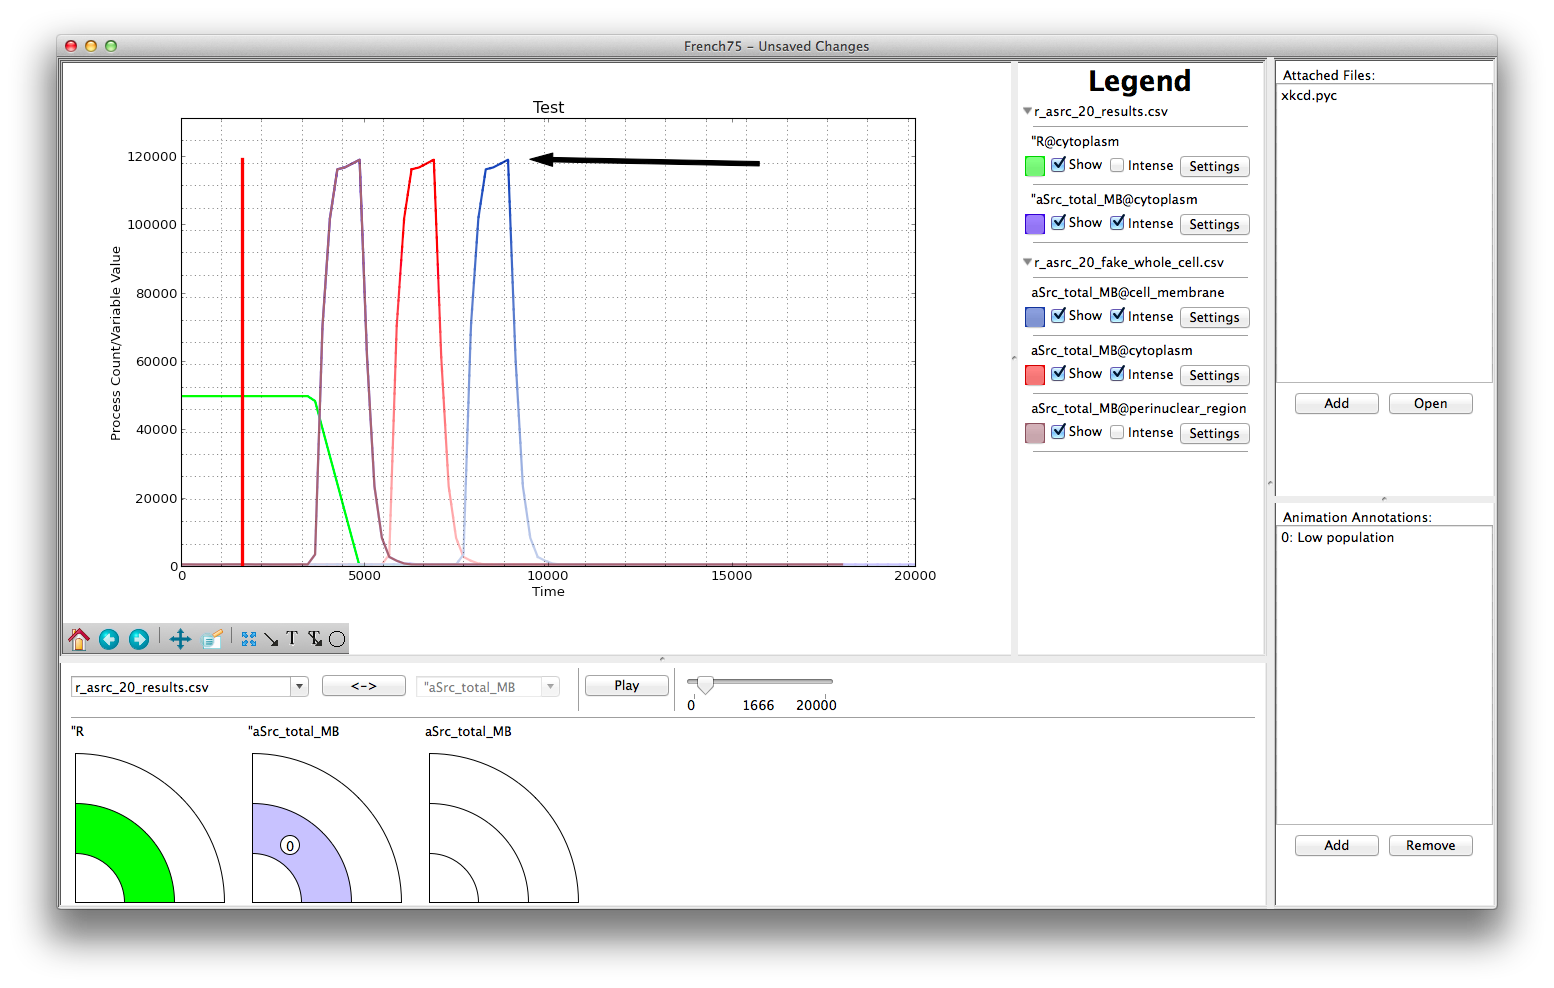
\includegraphics[width=\textwidth]{images/main_ui.png}
    \caption{Final \ac{UI}}
    \label{fig:main_ui}
\end{figure}

\begin{figure}[h!]
    \centering
    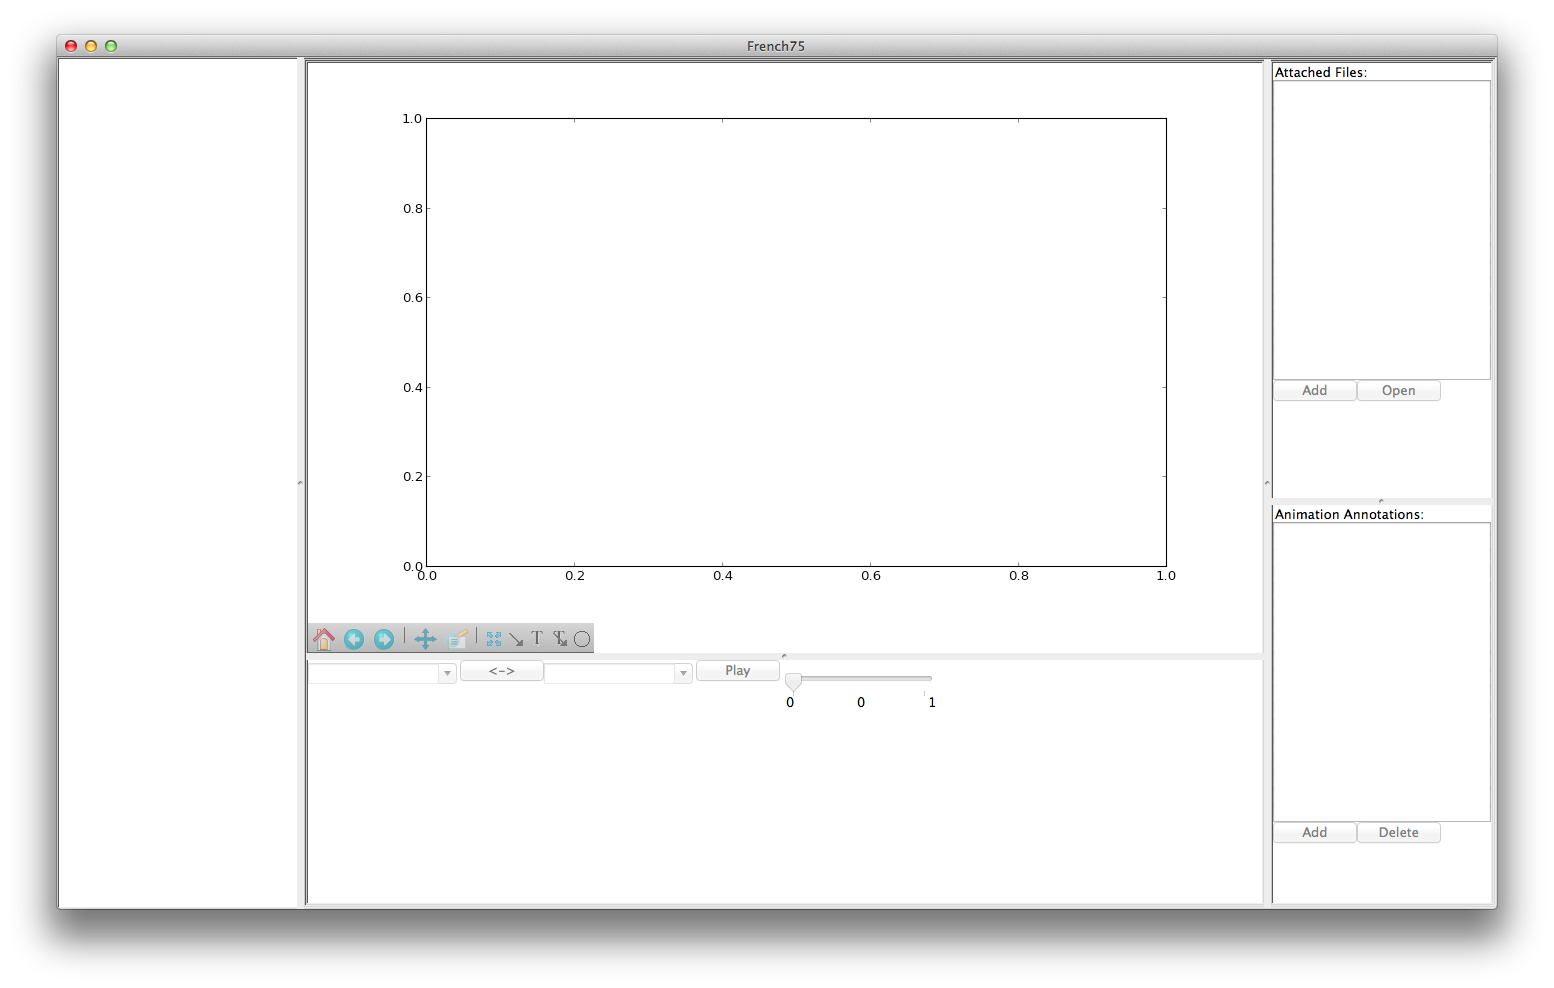
\includegraphics[width=\textwidth]{images/old_ui.png}
    \caption{Earlier \ac{UI}}
    \label{fig:old_ui}
\end{figure}

\begin{figure}[h!]
    \centering
    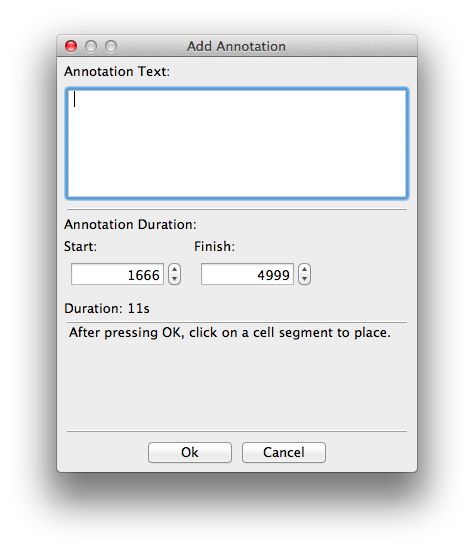
\includegraphics[width=0.5\textwidth]{images/add_annotation_dialogue.png}
    \caption{Add animation annotation dialogue}
    \label{fig:add_anime_annotation}
\end{figure}

\begin{figure}[h!]
    \centering
    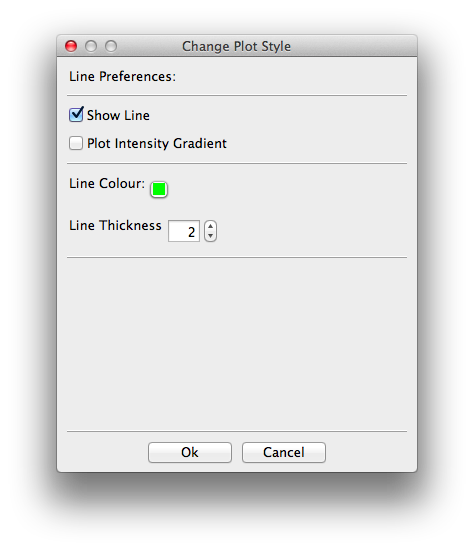
\includegraphics[width=0.5\textwidth]{images/plot_preferences_dialogue.png}
    \caption{Line preferences dialogue}
    \label{fig:plot_prefs_dialogue}
\end{figure}

\tdi{get figure of what session wizard used to look like}

\tdi{The bits below were blindly moved from work done.  They may need some changes to make them fit with evaluation}

\section{Usability}

In all the evaluations of the project users have commented on the difficulty of using parts of the tool.  Action has been taken to make it easier to use.  Many of the changes have been guided by Shneiderman~\cite{shgold}, Norman~\cite{normsev} \& Nielson's~\cite{neilten} guidelines.  Specifics are detailed below.

\subsection{Undo \& Redo}
\label{sec:undo}
Shneiderman calls for easy reversal of actions~\cite{shgold} and Nielson calls for user control and freedom -- an emergency exit from an unwanted state~\cite{neilten}.  To address this, undo/redo functionality has been added.  This required refactoring of the project code, so that the session data is in one location, inside a singleton (see Section~\ref{sec:design}). Any changes to this data are picked up during the next \ac{UI} update and are reflected in the visualisations.  The session data is stored as a dictionary.  To implement undo and redo, copies of the data dictionary are pushed and popped onto the stack.  Copies are pushed onto the undo stack on any atomic change the user makes.  This gives the user a full session history to go back through and this was one of the early goals from the first project phase.

A problem was encountered when trying to copy the dictionary onto the stack.  When pushing the dictionary onto the stack it would pushing a reference to the dictionary, not the dictionary itself. This meant that any changes to the dictionary after it had been pushed onto the stack were also there in the stack.  Python dictionaries have a copy method.  Copy only does a shallow copy -- any objects in the original dictionary will have their reference placed in the new dictionary.  This was fine for some parts of the session dictionary, but for others it was not. Lines and annotations, which are custom objects, presented problems.  This was solved by using Python's deep copy library.  With deep copy a new copy is made of objects as well.  Some elements of \texttt{wxPython} and \texttt{matplotlib} could not be deep copied, but this was fixed when the project architecture was changed to have the data in a single location.

\subsection{Saving}

It is important that a user is able to save and load the visualisation session as they may not be able to complete all their analysis in one sitting and may want to come back to their work in the future.  Without the ability to save and load the user would have to repeatedly add annotations, change preferences, and attach files.  It was possible to add saving and loading by building on the work done to implement undo \& redo, although further work was required. Python has a module called \texttt{pickle} to serialise and deserialise data.  When saving, the dictionary containing the centralised session data is pickled and written to a file and when loading the reverse happens.  Because the program is now focused on the data model, once a previous session has been loaded, a \ac{UI} refresh is triggered and the visualisation reflects the loaded data.

Saving the data also enables limited collaboration.  The user can customize the appearance and add annotations.  They can then save the state to a file and email that file to a colleague.  The colleague can then load the file and see the user's work.  The colleague can then correct any issues and add their own work.  The colleague can then save this and email it back to the user.  This is useful and is better than no collaboration, but it is entirely asynchronous.

\subsection{Feedback}
\label{sec:feedback}
Norman~\cite{normsev} and Shneiderman~\cite{shgold} both call for feedback to be given to the user so that the user can be sure that an action has been accomplished.  This feedback can come in a number of different forms and was in place in some parts of the project already.

Existing feedback in the project was a natural byproduct of some of the features; for example, when loading a results file the feedback that the load operation has been successful is that a graph appears on the screen. If the graph does not appear then something has gone wrong.  Additional feedback has been added to the project:
\begin{itemize}
\item When adding annotations the cursor changes to indicate to the user that they can interact with the graph in a different way.
\item The title bar text changes to display ``unsaved'' when the user makes a change and then changes back to ``saved'' when a successful save has been performed.
\end{itemize}

\subsection{Guiding the User}
\label{sec:guiding}

The first evaluation of the second phase of the project unearthed that the users struggled to choose the correct action as there were multiple ways of performing the same action that had slightly different use cases.  For example, at one point results files could be added via two different menu items.  There was also confusing language in the menu options.  These multiple paths have been removed. For example, now there is only one way to open results files initially.  To help guide the user further, \ac{UI} elements are enabled and disabled as appropriate.  Now when the program is first loaded the only action a user can perform is to load a session or start a new session, or join a session.  Afterwards other \ac{UI} elements are enabled to allow the user to start using the tool effectively.

To help guide the user when they first use the program a session wizard is created.  This replaced a series of separate menu items that the user previously had to navigate. The new session wizard would typically be the entry route in the first time a user runs the program.  It is therefore important that it helps them understand what it is they are doing.  The process of setting up the session should also be as easy as possible so that the user does not dislike the prospect of using the program.  The session wizard can be seen in Figure~\ref{fig:session_wizard}.

\begin{figure}[h!]
    \centering
    \begin{subfigure}[b]{0.4\textwidth}
        \centering
        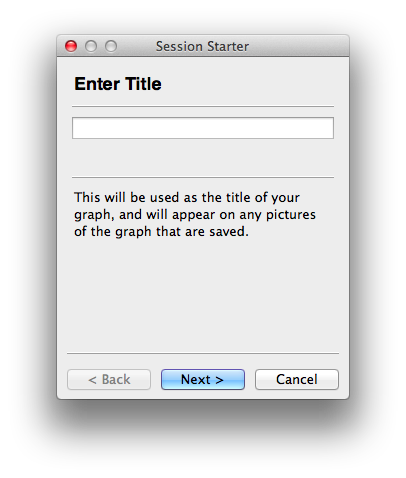
\includegraphics[width=\textwidth]{images/wizard_page_1.png}
        \caption{Wizard title chooser page}
        \label{fig:page_1}
    \end{subfigure}
    \begin{subfigure}[b]{0.4\textwidth}
        \centering
        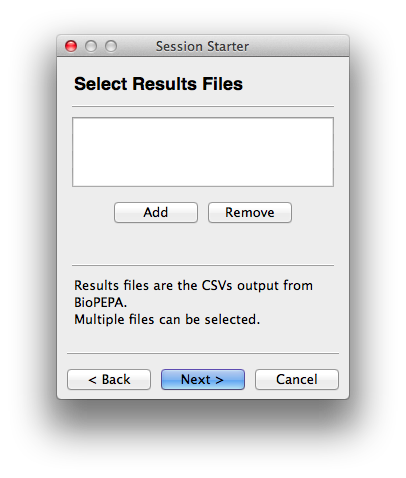
\includegraphics[width=\textwidth]{images/wizard_page_2.png}
        \caption{Wizard results selector page}
        \label{fig:page_2}
    \end{subfigure}

    \begin{subfigure}[b]{0.4\textwidth}
        \centering
        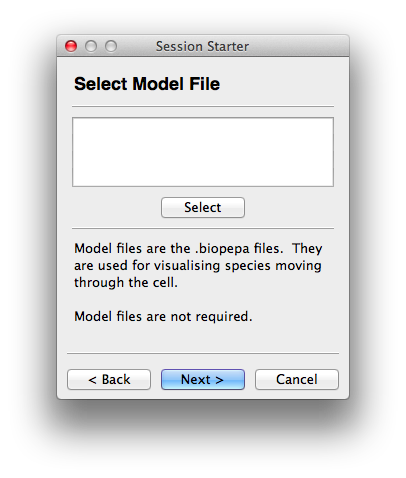
\includegraphics[width=\textwidth]{images/wizard_page_3.png}
        \caption{Wizard model selector page}
        \label{fig:page_3}
    \end{subfigure}
    \begin{subfigure}[b]{0.4\textwidth}
        \centering
        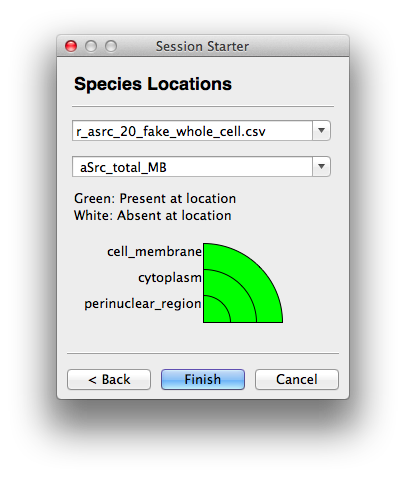
\includegraphics[width=\textwidth]{images/wizard_page_4.png}
        \caption{Wizard model viewing page}
        \label{fig:page_4}
    \end{subfigure}
    \caption{The session wizard that guides a user when setting up a session.}
    \label{fig:session_wizard}
\end{figure}

Form validators are used on the title fields and results fields.  The validators ensure that a title and at least one results file are included.  This stops the user from creating an invalid session.  There is also help text on each page of the wizard instructing the user on what actions they should take.

The model viewer page in Figure~\ref{fig:page_4} is similar to the cell cross-sections used in animation~\ref{sec:animation}.  There are two drop down boxes.  These drop down boxes control what is displayed in the cell cross-section.  Species in files can be selected.  The cell cross-section displays which compartments in the cell the species is present in.  The compartments are parsed from the model file.  This means that the model file is a requirement for model viewing and cell level animation.  This cell cross-section has replaced the previous model visualisation.  This model visualisation has two purposes. First, the user can sanity check that they have matching results and model files.  If a section of the cell has been left white then it acts as a cue to the user: if they were expecting the species to be present at that location then they know something has gone wrong.  Second, they can see how the model is structured.  The sections of the cell are labelled allowing the user to know what areas of the cell a species is present in.  This will hopefully increase their confidence with visualising and analysing the results from the models. Before the compartments were parsed from the model file automatically there was an user unfriendly system where the user had to input where in the cell a species is.  This was time consuming, difficult to use, and quite brittle.  At the time it assumed that there would be three compartments for every species, which is not a valid assumption.


\subsection{Matplotlib is Slow}

matplotlib is the de facto standard for graphing in Python this, amongst other reasons (detailed in the MPP report), led to it being chosen for the graph visualisations in the project.  When features such as plotting the intensity of the gradient were added matplotlib was pushed to its limits as it was being asked to plot hundreds of lines.  It was discovered that matplotlib is not optimised for speed, it is instead optimised for producing graphs of a publication standard.  This poses a dilemma: researchers want to be able to generate quality graphs, whilst the tool wants to offer real time interactivity and customisation.  There are tweaks that can be applied to make matplotlib be faster. There are also alternative graphing libraries that could be considered.  Threading was also looked into but caused segmentation faults.

\tdi{Became more noticable once collaboration was added and things were being redrawn more}


\subsection{Change how the visualisation is calculated}
Currently the visualisation is stored as a snapshot of the entire state.  The undo functionality is built around taking copies of this snapshot. When the visualisations are being displayed the \ac{UI} components look at this single snapshot.  Making copies of a large snapshot is not a cheap operation.  A more efficient approach would be to store operations.  To draw the latest visualisation the tool would simply traverse this list from the start.  Undoing an action would simply then be removing the last operation.

%\input{workplan}
\chapter{Conclusion}

This section contains a final look at the project.  The goals are re-examined and it is decided whether or not the project has met them.  There is also a detailed analysis of where future work in the project could be focussed.  Finally there is a discussion of the challenges that were faced and problems that could not be resolved.

\section{Comparison to Objective}
\label{sec:met_goal}

The aim of the project was: ``to develop a tool to visualise the results of dynamic time-series models of intra-cellular behaviour based on biochemical reactions".  This goal has been met.  The results can be visualised statically and dynamically.  The cell level visualisation applies domain knowledge familiar to biologists to help them understand their results.  Additional features to help the user work more efficiently and effectively have been added.  With respect to meeting the project goal the tool has been successful.

The user is able to interact with the visualisations.  They can customise them and attach additional information not present in the results files.

The user is also able to manipulate their data and export it.

Prototype features have been added for applying data mining techniques to allow the user to use their data to search databases of time series data and allowing users to collaborate in real time.

Evaluations with potential users have shown positive reception to this new tool and its features and a willingness to use this tool instead of the Eclipse plugin.

\section{Challenges Faced}

Some challenges were faced in this project that were not discussed elsewhere in this report.  These are presented below.

\subsection{wxPython Being Cross-Platform}
Python was chosen for this project to allow the project to be run on any system.  A cross platform \ac{GUI} toolkit was selected for the same reason.  \texttt{wxPython} was picked (details of why can be found in the MPP report).  At first this was successful.  The program was running on \texttt{MacOS} and \texttt{Linux}.  As the project was developed further some discrepancies were uncovered between \texttt{wxPython} on different platforms.  Initially this was coped with by writing different versions of parts of the code for each platform.  Eventually this became impractical.  Development support for \texttt{Linux} was halted.  Currently the project has only been tested running on \texttt{MacOSX} \texttt{Mountain} \texttt{Lion}.

An attempt was made to test the program on Windows, but there were problems installing the necessary Python libraries.

If this project was to be undertaken again, a different approach for the \ac{UI} would be chosen.  A browser based approach would be most suitable.  This is discussed Section~\ref{sec:cloud}.  \texttt{HTML} would become the primary source of the \ac{UI}.  The user's browser would render the \ac{UI}.  Different browsers should be able to render the same \ac{UI} on different platforms, as long as the \texttt{HTML} is standards compliant.

\section{Unsolved Problems}

\subsection{Complete Ordering Without Blocking}
\label{sec:ordering}

An initial version of collaboration used blocking communication.  In a blocking mode it was possible to globally order the events.  This is described in Section~\ref{sec:collaboration}.  Blocking collaboration is far from optimal.  A slow network would make the collaboration unusable.  The program would lock out the user for the duration of the message and response.  Non blocking communication was added later through the use of threads when sending messages.  Now a thread is spawned for each message sent between the client and the server.  This prevents the \ac{UI} from being locked out during the communication process.  This had the undesirable side effect of not being able to guarantee correct ordering.  No solution has been found for this, apart from switching to a centralised model as described in Section~\ref{sec:cloud}.

\subsection{Distributed Undo Forgetting States}

When doing a visualisation without any collaborators the undo and redo functionality works as expected.  In the collaborative mode however there is a bug.  If we have a user and a collaborator, changes the user makes are sent to the collaborator.  If the user issues an undo command their undo history is correct.  The collaborator's undo history appears to forget states.  This leaves the collaborator and the user seeing different visualisations.  This bug appears to be related to the issues that arose when first implementing undo and redo. Python's deep copy had to be introduced.  Despite numerous attempts to solve this bug a solution was not found that resolved the issue before the project deadline.

\section{The Future}

By the end of the project the program that had been developed was in a state that could be used by users.  There is more functionality than the Eclipse plugin and it is stable.  There is, however, work which could be done if development were to continue.  This is detailed below.

\subsection{Plots as Queries}
A prototype system for using plots as queries was developed (Section~\ref{sec:search}).  Early results are promising, but further work needs to be performed.  The first step would be working with a team of biologists and creating a large evaluation set. This would be a labelled set of plots that are similar or not similar.  This would allow the effectiveness to be accurately measured.  This would also include tuning of the parameters used, such as feature size and vocabulary size.  Other systems for using time series data as queries could also be developed and then the different systems can have their effectiveness compared.

There should also be an online repository of time-series data.  This would be processed for use in the search algorithms.  This would be done with the technique in Section~\ref{sec:search}.  \ac{tf.idf}, information retrieval, and machine learning in general, all rely on having a large amount of data.  One user will typically not have enough data to give the best results.  A central repository of data would allow all users' data to be used to gather statistics on the data to be used in the algorithms.  Other users' data could also be displayed in the results.  This would allow users to discover related work and potential collaborators.  Having a central repository also takes some control of the data out of the hands of the user.  Part of the reason for not integrating this feature with the \ac{UI} during this project was that it would have been difficult to track the location of the experiment data.  If the data had been uploaded to a central repository then there would be no problems tracking it, as the user would have no say in the location.

\subsection{More Data Mining and Machine Learning}

Enabling search was an early step into what can be done when machine learning and data mining is applied to time series data.  Other areas of interest include classification, clustering and anomaly detection~\cite{esling, chotirat}.  All of these can be built on top of the work that was done in Section ~\ref{sec:search}.

These are all features that would allow the user to analyse their work in a more detailed manner.

Again, all of these work best with a large amount of data and so would need to be tied into an online repository.

\subsection{Put it in the Cloud}
\label{sec:cloud}
All of the collaboration software reviewed (see Section~\ref{sec:review}) worked using a model where there is a single server.  This is a much simpler model for collaboration as the only ordering is the ordering on the server.

Adopting this model for the tool's architecture would require some refactoring of the project.  The code would need to be separated completely into a server and a client.  The server would do the the work: parsing the data, performing the intensity calculations and handling the creation of annotations.  The client would just display the information from the server.

Work towards this goal would also hopefully include rewriting the project so that the client could be a browser-based client.  A lot of problems arose from \texttt{wxPython} not being as cross platform compatible as had been hoped.  Rewriting the client to be browser-based should solve the cross platform problems.

The cloud backend would also, hopefully, include a repository for storing the attached files.  Currently there is no way for attached files to be sent to a collaborator.  They were considered too large to be sent through the implementation of collaboration described in Section~\ref{sec:collaboration}.  Without a central file repository we would need some other way of sending files.  This comes close to violating both Lett's and Zawinski's laws~\cite{atwood}.  These laws state, respectively, that all software evolves until it can send email and that all software evolves until it can read email.  They are a sign of feature creep in software.  Email would have been a potential solution on how to transfer the files between users, by building an email client into the program.  A central file repository avoids the need for this feature creep.  Previews of the files could be part of the real time features with thumbnails and title being transmitted.  The collaborators can upload and download the full file as necessary.

\subsection{Improve the Architecture}
\label{sec:conc_architect}

In Section~\ref{sec:architecture} the initial lack of architecture is discussed.  The architecture was improved and now resembles a \ac{MVC} architecture.  This work on the architecture should be continued in the future.  Making the architecture fully \ac{MVC} would greatly enhance the work towards moving the tool to the cloud (Section~\ref{sec:cloud}).

Having a \ac{MVC} architecture would also make it much easier to change interfaces.  New \acp{UI} could be developed and just connected to the model which would be running in the cloud.

\subsection{More Customisation}
Currently, the user is given control over the appearance of lines on the graph.  This could be expanded further into the tool.  Currently annotations cannot be customised, they can only be black.  More annotation options could be offered.  Also, different normalisation methods could be included as discussed in Section~\ref{sec:normalised}.

\subsection{More collaboration}
In addition to changing the model of collaboration from being distributed to centralised, further work should be done towards enabling communication between users.  Currently collaborators will have to use a phone or an external chat client to discuss the work.  A chat client could be integrated into the program.  This would enable communication without needing to switch between applications.  This chat client could also be specialised to include features that would be relevant to visualising data.

\section{Final Remarks}

The goal which was ``to develop a tool to visualise the results of dynamic time-series models of intra-cellular behaviour based on biochemical reactions" has been met.  This has made it a suitable replacement for the Eclipse plugin.

On top of the visualisation functionality, a suite of innovative features have been implemented to allow users to analyse their data quicker and more effectively.  They are also now able to collaborate in real time.

The functionality now offered by the tool is unique in the field.  No other software aimed at biologists allowed for real time collaboration, and no software allowed them to use their data to find similar data.

There is work required in these innovative features before they are fully ready for the user, but the effectiveness of these of the prototypes demonstrate the potential.  The new software can be considered a significant improvement for biologists.

The tool is going to be open sourced to allow others to continue the work that was undertaken.


\clearpage
%\appendix
%\addcontentsline{toc}{section}{Appendix}
%\input{wxmplexample}


%\clearpage
\addcontentsline{toc}{section}{References}
\bibliographystyle{unsrt}
\bibliography{biblio}


\end{document}
